\documentclass[journal]{IEEEtran}

% *** MISC UTILITY PACKAGES ***

\newcommand{\note}[1]{\textcolor{magenta}{#1}} 

\usepackage{silence} 
\WarningsOff[fixltx2e]

\usepackage[switch]{lineno}
\renewcommand{\linenumberfont}{\normalfont\bfseries\small\color{lightgray}}

% references
\usepackage[nocompress]{cite}
\usepackage[]{footmisc}
\usepackage{bookmark}

% *** GRAPHICS RELATED PACKAGES ***
\usepackage{graphicx}
\graphicspath{{./figures/}}

% *** MATH PACKAGES ***
%% with other math-related packages, you may want to disable it.
\usepackage{amsmath, amsthm, amsfonts,amssymb,eulervm,xspace, mathtools}
\usepackage{stmaryrd}%mapsfrom 
%\renewcommand{\restriction}{\mathord{\upharpoonright}} %restriction w/p space
\usepackage{mathrsfs} % math script fonts
\usepackage{relsize} %bigger
\usepackage{bm}

% theorem environments
\theoremstyle{definition}
\newtheorem{definition}{Definition}[section]
\newcommand{\definitionautorefname}{Definition}
\theoremstyle{remark}
\newtheorem{example}{Example}[section]
\newtheorem{axiom}{Axiom}
\newtheorem{prop}{Proposition} 

% *** diagrams
\usepackage{tikz}
\usetikzlibrary{cd}


% *** SPECIALIZED LIST PACKAGES ***
\usepackage{xcolor}
\usepackage[utf8]{inputenc}

\usepackage[outputdir=.]{minted}
\setminted[python]{fontsize=\scriptsize, 
                   linenos,
                   numbersep=8pt, 
                   frame=lines,
                   autogobble,
                   framesep=3mm, 
                   breaklines=True} 
% *** ALIGNMENT PACKAGES ***
\usepackage{multicol}
\usepackage{array}
\usepackage{multirow}
\usepackage{tabulary} 
% IEEEtran contains the IEEEeqnarray family of commands

% *** SUBFIGURE PACKAGES ***
\usepackage[caption=false,font=normalsize,labelfont=sf,textfont=sf]{subfig}

% *** FLOAT PACKAGES ***
\usepackage{dblfloatfix}

% *** PDF, URL AND HYPERLINK PACKAGES ***
\usepackage{xurl} 


%\usepackage[inline]{showlabels}

\usepackage{notation} %notation conventions
% correct bad hyphenation here
%\hyphenation{}

\begin{document}
\linenumbers

\title{Topological Equivariant Artist Model for Visualization Library Architecture}
% author names and IEEE memberships
\author{Hannah~Aizenman, Mikael Vejdemo-Johansson, Thomas~Caswell, and~Michael~Grossberg,~\IEEEmembership{Member,~IEEE,}% <-this % stops a space
\IEEEcompsocitemizethanks{\IEEEcompsocthanksitem H. Aizenman and M. Grossberg are with the department of Computer Science, City College of New York. 
\protect\\
% note need leading \protect in front of \\ to get a newline within \thanks as
% \\ is fragile and will error, could use \hfil\break instead.
E-mail: haizenman@ccny.cuny.edu, mgrossberg@ccny.cuny.edu 
\IEEEcompsocthanksitem Mikael Vejdemo-Johansson is with the department of Mathematics, CUNY College of Staten Island.
\protect\\
E-mail: mvj@math.csi.cuny.edu
\IEEEcompsocthanksitem Thomas Caswell is with National Synchrotron Light Source II, Brookhaven National Lab 
\protect \\
E-mail: tcaswell@bnl.gov}% <-this % stops an unwanted space
\thanks{Manuscript received X XX, XXXX; revised X XX, XXXX.}
}


% for Computer Society papers, we must declare the abstract and index terms
% PRIOR to the title within the \IEEEtitleabstractindextext IEEEtran
% command as these need to go into the title area created by \maketitle.
% As a general rule, do not put math, special symbols or citations
% in the abstract or keywords.
\IEEEtitleabstractindextext{%
\begin{abstract}
The abstract goes here.
\end{abstract}

% Note that keywords are not normally used for peerreview papers.
\begin{IEEEkeywords}
%Computer Society, IEEE, IEEEtran, journal, \LaTeX, paper, template.
\end{IEEEkeywords}}


% make the title area
\maketitle
\IEEEpeerreviewmaketitle
\IEEEraisesectionheading{\section{Introduction}\label{sec:intro}}



\IEEEPARstart{V}{isualization} tools implement transforms of the form $data \rightarrow graphic$ and are expected to be structure preserving. Loosely, that means the mathematical properties of the data and how the points are connected to each other should be inferable such that  $graphic \rightarrow data$. For example, values read off a bar chart have to be equivalent to the values used to construct that chart. Motivated by wanting to make better tools, we use algebraic topology to describe how $data$ and a corresponding $graphics$ have the same underlying structure and we use category theory to describing under what conditions the visualization tool preserves that structure such that $graphic \leftrightarrow data$. 

Algebraic structures allow us to describe many types of inherent structure in a uniform manner, and category theory provides a rigorous framework for specifying the behavior and properties of structure and maps between structures. For example, our framework can encapsulate how a table and scatter plot and heatmap are different representations of the same data and track an observation from a datacube as a point along a time series and on a map and in a network. The algebraic structures can be translated into programmatic types, while the categorical descriptions translate to a functional design framework. Strong typing and function composition enable library developers to build complex components from simpler verifiable parts \cite{huHowFunctionalProgramming2015, hughesWhyFunctionalProgramming1989}. These  components can be built as a standalone library and integrated into existing libraries and we hope these ideas will help shape the reorganization of critical data visualization libraries, such as Matplotlib. 

The contribution of this paper is a methodology for describing structure, verifying structure preservation, and specifying the conditions for constructing a structure preserving map between data and graphics. This framework also provides guidance for the construction and testing of structure preserving visualization library components.

\section{Related Work}
\label{sec:related-work:continuity}


\begin{figure}[H]
  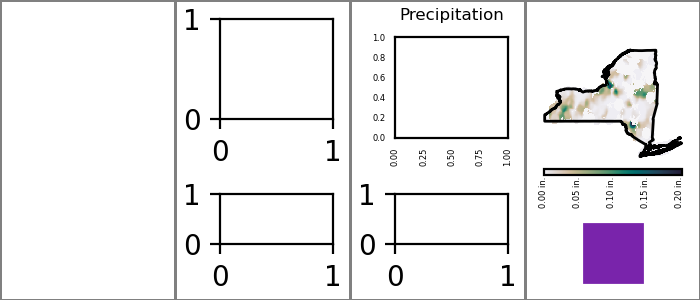
\includegraphics[width=1\columnwidth]{k_different_types.png}
  \caption{
  \note{add first panel which is table + all K type, second is scatter, etc...}
%
  \label{fig:related-work:continuity:ktypes}}
\end{figure}

Since the earliest maps \cite{friendlyBriefHistoryData2006}, a visualization has been expected to preserve the $field$ properties and $topology$ of the corresponding dataset; a \textcolor{fiber}{\textbf{field}} \footnote{Throughout this paper, we augment the math with color to group conceptually related terms\cite{headMathAugmentationHow2022}, for example \textcolor{fiber}{field} and \textcolor{fiber}{fiber}. This color coding carries through to the figures.}  is a set of values of the same type, e.g. one column of a table or the pixels of an image, and \textcolor{base}{\textcolor{topology}} is the connectivity and relative positioning of elements in a dataset \cite{wilkinsonGrammarGraphics2005}. In \autoref{fig:related-work:continuity:ktypes}, the topology is a continuous 3 dimensional surface encapsulating time and position, while the fields are date, location, station, pressure, and temperature. Our paper provides a language to express how the scatter plot, line plot, and heatmap are preserving different structural properties of the dataset, thereby generalizing Bertin's codification of how the topology of observations must match the class of representation (i.e. point , line, area) and how the variation possible in a field match the variation in the corresponding visual variable \cite{bertinSemiologyGraphicsDiagrams2011} and Mackinlay's work on how structure preservation includes preserving the mathimatical relations between elements of the same and different fields \cite{mackinlayAutomatingDesignGraphical1986}. 

While Bertin and Mackinlay's work primarily discusses the $data \rightarrow graphic$, Kindlemann and Scheidegger's algebraic framework \cite{kindlmannAlgebraicProcessVisualization2014} also dictates a set of conditions under which the $graphic \rightarrow data$  mapping is structure preserving. Encapsulating their conditions, we: present a uniform abstract data representation layer in \autoref{sec:atct:sheaves} for ensuring that the visualization should not change if the data representation (i.e. the data container) changes, define the conditions under which data maps unambiguously to visual elements \cite{ziemkiewiczEmbeddingInformationVisualization2009} in \autoref{sec:atct:xi}, and provide a methodology for verifying that changes in data should correspond to changes in the visualization in \autoref{sec:artist:equivariant:artist} that does not necessarily require that the changes be perceptually significant. Furthermore, our model extends their conditions of equivariance by explicitly incorporating topology and by providing a framework for translating the theoretical ideas into buildable components in \autoref{sec:construction}. 


\subsection{Fields} 
\label{sec:related-work:equivariance}
The structure on values has traditionally been described using the measurement scales-i.e. nominal, ordinal, interval, ratio - which Steven's classified by their mathematical group structure\cite{stevensTheoryScalesMeasurement1946} and others have formally expanded to include more types \cite{leaFormalizationMeasurementScale1971, thomasMathematizationNotMeasurement2014}. Specifically, Steven's conceptualizes the structure on values as \textcolor{action}{actions} on groups \footnote{A \textit{group} is a set with an associative binary operator, an identity, and an inverse operation}:

\begin{definition}\label{def:related-work:action}\cite{grimaldiDiscreteCombinatorialMathematics2006}
  An \textcolor{action}{\textbf{action}} of \textcolor{action}{$G = (G,\circ, e)$} on $X$ is a function  $act: \textcolor{action}{G} \times X \rightarrow X$. An action has the properties of identity $act(\textcolor{action}{e}, x) = x$ for all  $x \in X$ and associativity $act(\textcolor{action}{g}, act(\textcolor{action}{f}, x)) = act(\textcolor{action}{f} \circ \textcolor{action}{g}, x)$ for $\textcolor{action}{f},\textcolor{action}{g} \in \textcolor{action}{G}$.
\end{definition}

where the measurements are the groups and changes to them are actions. Structure preservetion in fields means that the data and the visualization are equivalent representations of an underlyng phenomena such that changes to data or visualization be reflected in the other in a consistent way. A function that preserves structure in this manner for groups is called equivariant. Given a group $G$ that acts on both the input $X$ and the output $Y$ of a function $f: X \rightarrow Y$
\begin{definition}
 A function $f$ is \textbf{equivariant} when $f(act(g,x)) = act(g,f(x))$ for all $g$ in $G$ and for all $x$ in $X$ \cite{pittsNominalSetsNames2013}
\end{definition}

which means that a visualization is structure preserving when there exist compatible actions on the data and visualization, as proposed by Kindlemann and Scheidegger\cite{kindlmannAlgebraicProcessVisualization2014}. Equivariance can sometimes be too restrictive because it can only be applied to groups and sometimes data does not have a group structure; an alternative is asserting that a visualization is structure preserving so long as it preserves the mathematical relations with and between fields, as proposed by Mackinlay\cite{mackinlayAutomaticDesignGraphical1987}, which is termed homomorphism. Given the function $f$ between sets $X$ and $Y$, both of which are equipped with the binary operator $\circ$
\begin{definition}
  
\end{definition}
  A function $f$ is \textbf{homeomorphic} when $f(x\circ y) = f(x) \circ f(y)$ for every pair of elements $x,y$ in $X$
\end{definition}
which means that applying the operation $\circ$ to the input to $f$ is equivalent to applying the operation to the output, which is only possibly when the output of the map $f$ from $X$ to $Y$ has the same structure as the input. Our framework for structure preservation incorporates equivariance and homomorphism and allows for defining other measures of equivalent representation; it is discussed in detail in \autoref{sec:artist:equivariant:data}. 

 
\subsection{Topology}
Borrowing strcutures from algebraic topology allows us to describe structure on individual elements in a way that holds true for the entire dataset, meaning we can use the same tools to check if structre is preserved regardless of whether the data fits in memory, is distributed, or is streaming. Our framework generalizesis because, informally, a topology $\mathcal{T}$ is a partitioning of a space into its subspaces in a way where those subspaces can be composed back into the space; the choice of partitions is how we encode the connectivity of the data and visualizations that we are interested in. 

\begin{definition}
A \textbf{topology} $\mathcal{T}$ on a space $X$ is a collection of open sets\footnote{Open sets (open subsets) are a generalization of open intervals to n dimensional spaces. For example, an open ball is the set of points inside the ball and excludes points on the surface of the ball. \cite{weissteinOpenSet,bradleyTopologyVsTopology}} \openset\ of $X$. This collection has the properties that the empty set $\varnothing$ and $\dbase$ are in $\mathcal{T}$, the union of open sets in $\mathcal{T}$ is also in $\mathcal{T}$, and any finite intersection of open sets in $\mathcal{T}$ is also in $\mathscr{T}$. \cite{bradleyTopologyCategoricalApproach2020}
\end{definition}

Visual algorithms assume the topology of their input data, as described in taxonomies of visualization algorithms Chi\cite{chiTaxonomyVisualizationTechniques2000} and by Troy and M\"{o}ller \cite{toryRethinkingVisualizationHighlevel2004}, but generally do not verify that input structure. For example, a \texttt{line} algorithm often does not have a way to query whether a list of (x,y) coordinates is the distinct rows, the time series, or the list of stations in \autoref{fig:related-work:continuity:ktypes}. While plotting the time series as a continuous line would be correct, it would be incorrect for a visualization to indicate that the distinct rows or stations are connected in a 1D continuous manner because it introduces ambiguity over which part of the line maps back to the data. A map that by definition has continous maps between two spaces, such as data and graphics, is called a homeomorphism\cite{riehlCategoryTheoryContext}. 

\begin{definition}
  A function $f$ is a $homeomorphism$ if it is bijective, continous, and has a continous inverse function f^{-1}. 
\end{definition}

To encode topology and field structure, we extend Butler's work on using a mathematical structure called fiber bundles as an abstract data representation in visualization \cite{butlerVectorBundleClassesForm1992, butlerVisualizationModelBased1989}. We sketch out fiber bundles in \autoref{sec:atct:fiber-bundles}, but Butler provides a thorough introduction to bundles for visualization practitioners.


\subsection{Structure Preservation In Software}
\label{sec:related-work:software}
Visualization libraries are in part measured by how expressive the components of the library are, where expressiveness is a measure of which structure preserving mappings a tool can implement \cite{mackinlayAutomatingDesignGraphical1986}. While some visualization tools aim to automate the pairing of data with structure preserving visual representations, such as Tableau\cite{StoltePolaris2002,hanrahanVizQL2006,MackinlayShowme2007}, many visualization libraries leave that choice to the user. For example, connectivity assumptions tend to be embedded in each of the visual algorithms of `building block` libraries, a term used by Wongsuphasawat \cite{wongsuphasawatNavigatingWideWorld2021} to describe libraries that provide modular components for building elements of a visualization, such as functions for making boxes or translating data values to colors. In building block libraries such as Matplotlib\cite{hunterMatplotlib2DGraphics2007} and D3\cite{bostockDataDrivenDocuments2011} the connectivity assumptions lead to very different interfaces; for example in Matplotlib methods for updating data and parameters for controlling aesthetics differ between plots. While VTK\cite{hanwellVisualizationToolkitVTK2015,geveciVTK2012} provides a language for expressing the topological properties of the data, and therefore can embed that information in its visual algorithms, it does so in a non-uniform manner. On the other hand, domain specific libraries are designed with the assumption of continuities that are common in the domain \cite{HeerSoftware2006}, and therefore can somewhat restrict the interface to choices that that are appropriate for the domain. For example, a tabular topological structure of discrete rows, as illustrated in \autoref{fig:related-work:continuity:ktypes}, is assumed by 
A Presentation Tool\cite{mackinlayAutomatingDesignGraphical1986, mackinlayAutomatingDesignGraphical1986} and grammar of graphics\cite{wilkinsonGrammarGraphics2005} and the ggplot\cite{wickhamGgplot2ElegantGraphics2016}, vega\cite{satyanarayanDeclarativeInteractionDesign2014}, and altair\cite{vanderplasAltairInteractiveStatistical2018} libraries built on these frameworks. Image libraries such as Napari\cite{nicholas_sofroniew_2021_4533308} and ImageJ\cite{schneiderNIHImageImageJ2012} and its humanities ImagePlot\cite{studiesCulturevisImageplot2021} plugin assume that the input is 2D continuous. Networking libraries such as gephi\cite{bastianGephiOpenSource2009} and networkx\cite{HagbergExploringNetwork2008} assume a graph-like structure. By assuming the structure of their data, these domain specific libraries can provide more cohesive interfaces for a much more limited set of visualization algorithms than the building block libraries offer. 
\note{transition sentence}
In this work, we formally specify the conditions necessary to build structure preserving components using category theory, because it provides a rich language for expressing the structure of objects, functions between objects, and the constraints that must hold for these functions to compose \cite{wielsManagementEvolvingSpecifications1998,yorgeyMonoidsThemeVariations2012}. A brief visualization oriented introduction to category theory is in Vickers et al \cite{vickersUnderstandingVisualizationFormal2013}, but they are applying category theory to semantic concerns about visualization design rather than library architecture. 


\section{Formal Properties of Data \& Graphics}
\label{sec:atct}
In this section, we propose a mathematical abstraction of the data input and graphic pre-rendered output. This mathematical abstraction has a robust language for expressing topology and fields; expresses how to verify that data continuity is preserved on subset, distributed, and streaming data representations; and formalizes the expectation of a correspondence between data and visual elements. 

\subsection{Abstract Data Representation}
\label{sec:atct:fiber-bundles}
We model data using a mathematical representation of data that can encode topological properties, field types, and data values in a uniform manner using a structure from algebraic topology called a fiber bundle. We extend Butler's proposal of bundles as abstract visualization data type \cite{butlerVectorBundleClassesForm1992,butlerVisualizationModelBased1989} by incorporating Spivak's methodology for encoding named data types from his fiber bundle representation of relational databases \cite{spivakDatabasesAreCategories2010,spivakSimplicialDatabases2009}. We build on this work to describe how to encode the connectivity of the data as a topological space, separately encode the fields as their own topological space with a typing system, and express the mappings between these two spaces.

The fiber bundle abstraction is a structure fusing some \textcolor{base}{base space} (indexing into the data) with some \textcolor{fiber}{fiber space} (acting as the data domain). This sort of fusion could be done by a simple direct product (or join-operation), but with the fiber bundle abstraction we get the flexibility of expressing more complicated fusions than the direct product, as long as they can be constructed from building blocks that look like direct products.

\begin{definition}\label{def:fiber_bundle}
   A \textbf{fiber bundle} $(\dtotalc, \dbasec, \pi, \dfiberc)$ is a structure with topological spaces $\dtotalc, \dfiberc, \dbasec$ and  bundle projection map $\pi: \dtotalc \rightarrow \dbasec$ \cite{FiberBundle2020,spanier1989algebraic}. 
\begin{equation}
  \label{eq:atct:fb:intro}
  \begin{tikzcd}[ampersand replacement=\&, row sep=huge]
   \dfiberc
    \arrow[r, hook, color=total] \& 
    \dtotalc
    \arrow[d, "\pi"',color=total, two heads] \\
     \& 
  \dbasec
     \arrow[u, "\dsectionc"', bend right, pos=.5, color=section, dashed]
  \end{tikzcd}
\end{equation} 
A continuous surjective map $\bm{\pi}$ is a \textbf{bundle projection} map when 
\begin{enumerate}
  \item all fibers in the bundle are isomorphic. Since all fibers are isomorphic, there is a uniquely determined \textcolor{fiber}{fiber space} \dfiberc\ given by the preimage of the projection $\pi$ at any point $\dbasepoint$ in the \textcolor{base}{base space} \dbasec: $\dfiberc = \pi^{-1}(k)$.  
  %the \textcolor{fiber}{fiber space} \dfiberc\ is the preimage of the projection function $\pi$ at a point $\dbasepoint$ in the \textcolor{base}{base space} \dbasec\ such that $\dfiber_{\dbasepoint} = \pi^{-1}(\dbasepoint)$. All fibers in a bundle are isomorphic such that $\dfiber \cong \dfiber_{\dbasepoint}$ for all points $\dbasepoint \in \dbase$. 
  \item each point $\dbasepointc$ in the \textcolor{base}{base space} \dbasec\ has an open neighborhood $\openset_{\dbasepointc}$ such that the \textcolor{total}{total space} \dtotalc\ over the neighborhood is locally trivial. \textbf{Local triviality} means $\dtotal\restriction_{\openset} = \openset\times F$. In this paper we use $\dtotal\restriction_{\openset} = \pi^{-1}(\openset)$ to denote the preimage of an openset, and a \textbf{local trivialization} is a specific choice of neighborhoods and their preimages.
  %there is an open neighborhood $\openset_{\dbasepoint}$ surrounding each point in the base space $\dbasepoint \in \openset_{\dbasepoint} \subset \dbase$ such that the \textcolor{total}{total space} \dtotalc\ over the neighborhood, denoted $\dtotal\restriction\openset$\footnote{The symbol $\restriction$ is the restriction operator\cite{RestrictionMathematics2022} defined in \texttt{amssymb}. For example $\pi^{-1}\restriction\openset$ is the inverse function $\pi^{-1}$ defined only on the points in $\openset$. Since $\pi^{-1}(\dbase)=\dtotal$, we use the shorthand $\dtotal\restriction_{\openset} \coloneqq \pi^{-1}\restriction_{\openset}$}, is locally trivial. The condition for local triviality is that $\dtotal\restriction_{\openset} = \openset \times \dfiber = \pi^{-1}\restriction_{\openset}$
\end{enumerate}
\end{definition}
\begin{definition} A \textcolor{section}{\textbf{section}} $\dsectionc: \dbasec \rightarrow \dtotalc$ over a fiber bundle is a smooth right inverse of $\pi$: $\pi(\dsection(\dbasepoint)) = \dbasepoint$ for all $\dbasepoint \in \dbase$
\end{definition}

\begin{figure}[H]
  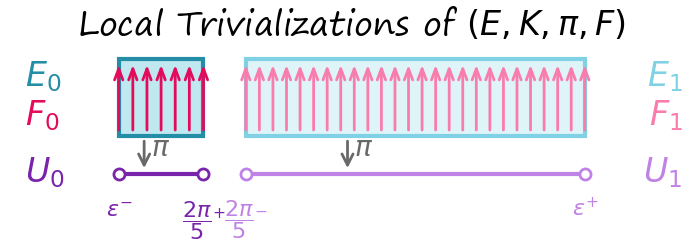
\includegraphics[width=\columnwidth]{figures/local_trivalizations.png}
  \caption{The local trivializations $\dtotal_{0}$ and $\dtotal_{1}$ are subspaces of $\dtotal$ where the fibers $\dfiber_{0}$ are equal, here illustrated as all pointing in the same direction. These local trivializations are themselves locally trivial fiber bundles.} 
  \label{fig:atct:local_trivalizations}
\end{figure}

\note{Add motiviating note here!}
Consider the circle. Points can be identified with angles (in radians, for instance), and we can imagine covering the circle with two overlapping intervals - for instance $\dbase_0=(-\varepsilon, 2\pi/5+\varepsilon)$ and $\dbase_1=(2\pi/5-\varepsilon, 2\pi+\varepsilon)$. We can imagine creating building blocks $\dbase_0\times[-1,1]$ and $\dbase_1\times[-2,2]$.

There are two different ways to create a fiber bundle that has these building blocks as the local trivializations: on the one hand, we could imagine just a cylinder $S^1\times[-1,1]$ as a total space. The fibers would all be just the interval $[-1,1]$. Over $\dbase_0$, we could map from the local trivialization to the total space with the identity map, and over $\dbase_1$ we could map from the local trivialization to the total space by rescaling the fiber space $[-2,2]\to[-1,1]$.

On the other hand, we could imagine creating a Möbius strip by flipping one end of $\dbase_1\times[-2,2]$ over before attaching it, so that while $\dbase_0\times[-1,1]$ gets mapped into the total space with the identity map, the part $(2\pi-\varepsilon,2\pi+\varepsilon)\times[-2,2]$ of $\dbase_1\times[-2,2]$ is mapped by the function $x\mapsto -x/2$ instead of the function $x\mapsto x/2$.

These functions - using the isomorphisms $x\mapsto x$, $x\mapsto x/2$ and $x\mapsto -x/2$ to map from each rectangle into the cylinder compose into different maps $(\dbase_0\cap\dbase_1)\times[-2,2]\to(\dbase_0\cap\dbase_1)\times[-1,1]$ where the source is seen as a subset of $\dbase_1\times[-2,2]$ and the target is seen as a subset of $\dbase_0\times[-1,1]$. By specifying just these \textbf{transition maps} for all overlaps of cover elements in the local trivialization we can specify a gluing scheme that constructs the fiber bundle from these locally trivial pieces.


%For example, in \autoref{fig:local_trivalizations}, the bundles $\dtotal_{0}=\dtotal\restriction_{[\epsilon^{-}, {\frac{2\pi}{5}}^{+}]}$ and $\dtotal_{1}=\dtotal\restriction_{[{\frac{2\pi}{5}}^{-}, \epsilon^{-}]}$ are local trivializations of an arbitrary bundle $\dtotal$. These local trivializations overlap on the intersections of the open subsets of each trivialization $[\epsilon^{-}, \epsilon^{+}]$ and $[{\frac{2\pi}{5}}^{-}, {\frac{2\pi}{5}}^{+}]$. A set of trivializations can be glued into a larger bundle by defining transition maps that describe how to align the fibers in the overlapping space such that the sections of the bundle remain continuous. 
\note{add transition map construction formula} 

\begin{figure}[H]
  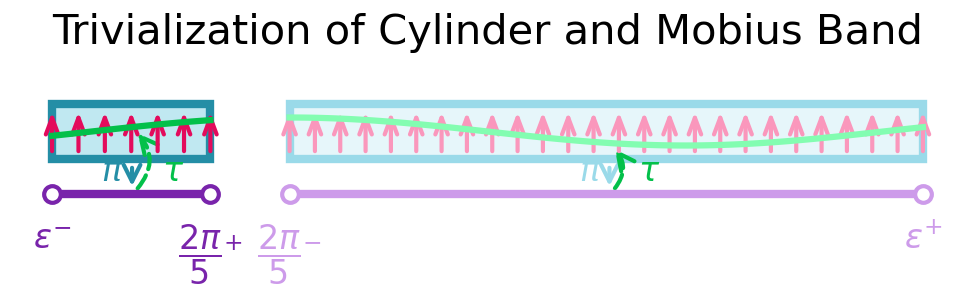
\includegraphics[width=1\columnwidth]{figures/cyl_mob.png}
  \caption{\note{figure out short caption here}\label{fig:cyl_mob_bundles}}
\end{figure}
As demonstrated in \autoref{fig:cyl_mob_bundles} different types of total spaces can be decomposed into the same local trivializations; therefore the distinguishing factor between total spaces can be the transition maps for constructing the spaces from trivializations. 

A \textit{trivial bundle} is directly isomorphic to $\dbasec\times\dfiberc$, and for any choice of cover of $\dbasec$ by overlapping opensets, we can choose local trivializations so that all transition maps are identity maps. In the example in Figure~\ref{fig:cyl_mob_bundles}, we use arrows $\uparrow$ to denote fiber alignments, illustrating that by choosing simple enough trivializations, we get identity maps in the transition maps.

%In a \textit{trivial bundle}, the fibers are identical $\dfiber = \dfiber_{k}$ for all points $\dbasepoint \in dbase$ such that all the transition maps are also identical. For example, in the cylinder case the fibers in the overlapping regions of the trivializations point in the same direction $\uparrow$ to illustrate that they are equal $\dfiber_0\restriction_{\openset_1\cap\openset_2} = \dfiber_{1}\restriction_{\openset_1\cap\openset_2}$. Because the fibers point in the same direction, the  transition maps at both intersections map the fiber to itself $\uparrow\rightarrow\uparrow$.

A \textit{non-trivial bundle} on the other hand is one that can not be constructed as $\dbasec\times\dfiberc$, but where the construction is more complicated. Then for any choice of local trivializations, there is at least one transition map that is not an identity \cite{hatcherAlgebraicTopology2002}. For example, in the Möbius band case, while $\dfiber_0\restriction_{(2\pi/5-\varepsilon, 2\pi/5+\varepsilon)}\to\dfiber_1\restriction_{(2\pi/5-\varepsilon, 2\pi/5+\varepsilon)}$ can be chosen to be an identity map (after transforming $\dbase_1\times[-2,2]\to\dbase_1\times[-1,1]$ by rescaling), the other transition map component $\dfiber_0\restriction_{(-\varepsilon,\varepsilon)}\to\dfiber_1\restriction_{(-\varepsilon,\varepsilon)}$ has to flip the fibers to align them between the pieces.


We propose that the total space of a bundle can encode the mathematical space in which a  dataset is embedded, the base space can encode the topological properties of the dataset, and the fiber space can encode the data types of the record fields of the dataset. The map $\pi$ expresses the formal binding between having a typed data field, discussed in \autoref{sec:atct:fb:fiber}, and a corresponding point in the topological structure, which is discussed in \autoref{sec:atct:fb:base}. Fiber bundles are a good abstract data representation for visualization because the field type and topological structure are unconstrained in terms of dimensionality and the only conditions that must be satisfied are that every point in the base space has a corresponding field of values and the field types must be the same for every point in the base space. We propose that modeling data as sections provides a way to encapsulate topological and field structure in a uniform dimension and type independent manner, as discussed in \autoref{sec:atct:fb:sections}.

\subsubsection{Topological Structure: Base Space \dbase}
\label{sec:atct:fb:base}
\note{base space of bundle for key/value pair, topology in general 'cause data + viz continuity in same way}
Munzner~\cite{munznerChDataAbstraction} describes a key-value semantics for data representation and abstraction, where datasets can be queried with different kinds of keys depending on the dataset type - locations for values of spatial fields, times for values of time series, or indexes for values in flat or multidimensional tables.
We propose that these different types of keys are instances of different underlying topological organization of the data, and that we can use the structure of the opensets in the topological space to encode the extent to which the keys can vary continuously: flat or multidimensional tables have discrete points as indices, time series have points on a line as indices and spatial fields (regardless of whether they are scalar or tensor fields) have points in a spatial domain as indices. Therefore we choose to encode the topological structure of the data as the \textcolor{base}{base space} of a fiber bundle. Because the base space of a fiber bundle is a quotient topology\cite{munkresElementsAlgebraicTopology1984}, it divides the topological space into the largest number of open sets such that $\pi$ remains a continuous function. This means that the topology can be defined to have a resolution equal to the number of indices in a dataset such that the key (continuity)-value (data) pairing is always preserved. 

Following from Spivak's categorical abstraction of a database \cite{spivakSimplicialDatabases2009,spivakDatabasesAreCategories2010}, we also propose that the structure of the data types be formally specified as the objects of a category.

\begin{definition}\label{def:atct:category}
   An \textbf{category} $\mathcal{C}$ consists of the following \textit{data}: 
\begin{enumerate}
  \item a collection of \textit{objects} $X \textbf{ob}(\mathcal{C})$
  \item for every pair of objects $X, Y \in \textbf{ob}(\mathcal{C})$, a set of \textit{morphisms} $X \xrightarrow{f} Y \in Hom_{\mathcal{C}}(X, Y)$
  \item for every object $X$, a distinct \textit{identity morphism} $X \xrightarrow {id_x} X$ in $Hom_{\mathcal{C}}(X, X)$
  \item a \textit{composition function} $f \in Hom_{\mathcal{C}}(X, Y) \times  g \in Hom_{\mathcal{C}}(Y, Z) \rightarrow g \circ f \in Hom_{\mathcal{C}}(X, Z)$
\end{enumerate}
such that 
\begin{enumerate}
  \item \textit{unitality:} for every morphism $ X \xrightarrow{f} Y$, $f \circ id_x = f = id_y \circ f$
  \item \textit{associativity:} if any three morphisms $f, g, h$ are composable, 
    \begin{equation*}
      \begin{tikzcd}
        X \arrow[r, "f"] \arrow[rrr, "h\circ(g\circ f) = (h\circ g)\circ f"', bend right, dashed] & Y  \arrow[r, "g"] & Z \arrow[r, "h"] & W
        \end{tikzcd}
  \end{equation*}
  then they are associative such that $h\circ(g\circ f) = (h \circ g) \circ f$  \cite{lawvere2009conceptual,riehlCategoryTheoryContext,maclaneCategoriesWorkingMathematician2013,fongInvitationAppliedCategory2019}. 
  \end{enumerate}
\end{definition}

The standard construction of a category from a topological space is that it has open set objects $\opensetc$ and inclusion morphisms $\opensetc_i \xrightarrow{\iota} \opensetc_j$ such that $\opensetc_i \subseteq \opensetc_j$\cite{riehlCategoryTheoryContext}. The composability property expresses that inclusion is transitive, while associativity expresses that the inclusion functions can be curried in various equivalent groupings. By formally specifying the properties of the topological structure data types as $\mathcal{\dbase}$, we can express that these are the properties that are required as part of the implementation of the data type objects. 

For example, the disjoint union of two bundles, as shown in \autoref{fig:atct:local_trivalizations}, is the coproduct $\dbase^{a} \subseteq_{\dbase^{c}} \dbase^{b}$ over an overlap $\dbase^{c}$ and therefore the inclusion morphism must be commutative:
\begin{figure}
  \includegraphics*[width=1\columnwidth]{figures/tex/k_coproduct.pdf}
\end{figure}

The coproduct in \autoref{eq:atct:base_union} shows that the way to test that two spaces have been combined correctly is to verify that every point in the subspace $\dbasepoint \in \dbase^{c}$ must be present in the spaces for which inclusion morphisms exist $\dbasepoint \in \dbase^{a}$ and $\dbasepoint \in \dbase^{b}$ such that $\dbasepoint \in \dbase^{a}\sqcup_{\dbase^{c}} \dbase_{b}$. This simple test that the records are joined correctly is what allows us to reliably build larger datasets out of smaller ones, such as in the case of distributed and on demand datasets.


\subsubsection{Data Field Types: Fiber Space \dfiber}
\label{sec:atct:fb:fiber}
As mentioned in \autoref{sec:related-work:equivariance}, visualization researchers traditionally describe equivariance as the preservation of field structure, which is based on the field type. Spivak shows that data typing can be expressed in a categorical framework in his fiber bundle formulation of tables in relational databases \cite{spivakDatabasesAreCategories2010,spivakSimplicialDatabases2009}. In this work, we adopt Spivak's definitions of \textit{type specification}, \textit{schema}, and \textit{record} because that allows us to use a dimension agnostic named typing system for the fields of our dataset that is consistent with the abstraction we are using to express the continuity. Spivak introduces a \textit{type specification} as a bundle map $\pi: \mathscr{U} \rightarrow \textbf{DT}$. The base space $\textbf{DT}$ is a set of data types $T \in \textbf{DT}$ and the total space $\mathscr{U}$ is the disjoint union of the domains of each type \[\mathscr{U} = \bigsqcup_{T \in \textbf{DT}} \pi^{-1}(T)\] such that each element $x$ in the domain $\pi^{-1}(T)$ is one possible value of an object of type $T$ \cite{spivakSimplicialDatabases2009}. For example, if $T=\texttt{int}$, then the image $\pi^{-1}(\texttt{int}) = \mathbb{Z} \subset \mathscr{U}$ is the set of all integers and $x=3 \in \mathbb{Z}$ is the value of one $\texttt{int}$ object. 

Since many fields can have the same datatype, Spivak formally defines a mapping from field name to field data type, akin to a database schema \cite{ullmanFirstCourseDatabase2008}. According to Spivak, a \textit{schema} consists of a pair $(\fnames, \sigma)$ where $\fnames$ is the set of field names and $\sigma: \fnames \rightarrow \textbf{DT}$ is a function from field name to field data type\cite{spivakSimplicialDatabases2009}. The function $\sigma$ is composed with $\pi$ such that $\pi^{-1}(\sigma(C)) \subseteq \mathscr{U}$; this composition induces a domain bundle $\pi_{\sigma}:\mathscr{U}_{\sigma} \rightarrow \fnames$ that associates a field name $c \in C$ with its corresponding domain $\pi^{-1}_{\sigma}(C) \subseteq \mathscr{U}_{\sigma}$. 
\begin{definition} A \textbf{record} is a function $\delement: \fnames \rightarrow \mathscr{U}_{\sigma}$ and the set of records on $\pi_{\sigma}$ is denoted $\Gamma^{\pi}(\sigma)$. Records must return an object of type $\sigma(\fname) \in \textbf{DT}$ for each field $c \in C$.
\end{definition}
Spivak then describes tables as sections $\dsection: \dbase \rightarrow \Gamma^{\pi}(\sigma)$ from an indexing space $\dbase$ to the set of all possible records $\Gamma^{\pi}(\sigma)$ on the schema bundle, and his notion of a table generalizes to our notion of a data container. 

To build on the rich typing system provided by Spivak, we define the \textcolor{fiber}{fiber space} \dfiberc\ to be the space of all possible data records
\begin{equation}
  \dfiberc \coloneqq \{\delement: \fnames \rightarrow \mathscr{U}_{\sigma} \bigm{\vert} \pi_{\sigma}(\delement(\fname)) = \fname\;for\;all\; \fname \in \fnames \}
\end{equation}
such that the preimage of a point is the corresponding data type domain $\pi^{-1}(\dbasepoint) = \dfiber_{k} = \mathscr{U}_{{\sigma}_{\dbasepoint}}$. 
Adopting Spivak's fiber bundle construction of types allows our model to reuse types so long as the field names are distinct and that field values can be accessed by field name,  since those are sections on $\mathcal{U}_{\sigma}$. Furthermore, since domains $\mathscr{U}_{{\sigma}}$ of types are a mathematical space, multi-dimensional fields can be encoded in the same manner as single dimensional fields and fields can have different names but the same type. 

As with the base space category $\mathcal{\dbase}$, we propose a fiber category $\mathcal{\dfiberc}$ to encapsulate the field types of the data. The fiber category has a single object $\dfiberc$ of an arbitrary type and morphisms on the fiber object $\dfunctc \in Hom(\dfiberc, \dfiberc)$. We can also equip the category with any operators or relations that are part of he mathematical structure of the field type. For example we can equip the category with a comparison operator, which is part of the definition of the monoidal structure of a partially ordered ranking variable \cite{bruggemannRankingPrioritizationMultiindicator2011} or the group structure of Steven's ordinal measurement scale \cite{stevensTheoryScalesMeasurement1946, leaFormalizationMeasurementScale1971, thomasMathematizationNotMeasurement2014}. Steven's other scales are summarized in \autoref{tab:appendix:summary:stevens}. 

The fiber category $\mathcal{\dfiberc}$ is also equipped with a bifunctor because it is a monoidal category and this functor provides a method for combining fiber types. The bifunctor $\otimes: \mathcal{\dfiber} \times \mathcal{\dfiber} \rightarrow \mathcal{\dfiber}$ allows us to express fields that contain complexly typed values. For example, wind can be represented as two fields $\dfiber_{speed} \times \dfiber_{direction}$ or a composite fiber field $\dfiber_{speed} \otimes \dfiber_{direction} = \dfiber_{wind}$. The $\otimes$ encapsulates both the sets associated with each fiber $\mathbb{R} \times \mathbb{R} = \mathbb{R}^{2}$ and the morphisms associated with each functor $(\dfunct_{speed}, \dfunct_{direction}) = \dfunct_{wind}$. Combining fibers can be verified by checking that when a fiber component $\dfiber^{c}$ is present in both $\dfiber^{a}$ and $\dfiber^{b}$, it is identical when projected out of either such that the *product* diagram commutes:

\begin{figure}
  \includegraphics*[width=1\columnwidth]{figures/tex/f_product.pdf}
\end{figure}

\note{this is really a bookkeeping thing - each field is at an index/ splitting a field shouldn't change values} This means that data with many fields is decomposed into its component fields, shared records stay the same. For example, the red (temperature, time, pressure) record separates into (temperature, time) and (pressure, time) records that share the same red time. Furthermore this time is the same whether it is obtained from the (temperature, time) or (pressure, time) record. This simple test that fields are joined together correctly for the same record is what allows us to reliably combine multiple datasets together on shared properties-for example growing the weather station data from a temporal to spatial dataset by adding the weather at each  location at each time. 

\subsubsection{Data: Section} 
\label{sec:atct:fb:sections}
We encode data as a \textcolor{section}{section} \dsectionc\ of a bundle because this allows us to incorporate the topology and field types in the data definition. We can define these section functions locally, meaning that the section is (piece-wise) continuous over a specific open subset \openset\ of \dbase\
\begin{equation}
  \label{eq:atct:fb:sections}
  \cgamma{\opensetc}{\dtotalc\restriction_{\opensetc}} \coloneqq \big\{\dsectionc: \opensetc\rightarrow \dtotalc\restriction_{\opensetc} \; \bigm{\vert} \pi(\dsectionc(\dbasepointc)) = \dbasepointc\;for\, all\; \dbasepointc \in \opensetc \big\} 
\end{equation}
such that each section function $\dsection: \dbasepoint \mapsto \delement$ maps from each point $\dbasepoint \in \openset$ to a corresponding record in the fiber space $\delement \in \dfiber_{\dbasepoint}$ over that point. Bundles can have multiple sections, as denoted by $\Gamma(\openset, \dtotal\restriction{\openset})$. We can therefore model data as structures that map from an index like point $\dbasepoint$ to a data record $\delement$, and encapsulate multiple datasets with the same fiber and base space as different sections of the same bundle. 

In a trivial bundle, the total space is the product of the fiber and base space $\dtotalc = \dbasec \times \dfiberc$. This allows us to define global sections $\dsection: \dbase \rightarrow \dfiber \in \Gamma(\dbase, \dfiber)$ which we translate into a data signature of the form  
\begin{equation}
  \textcolor{section}{\texttt{dataset}}: \textcolor{base}{\texttt{topology}} \rightarrow \textcolor{fiber}{\texttt{field}}
\end{equation}
where $\dsection=\texttt{dataset}$, $\dbase=\texttt{topology}$ and $\dfiber=\texttt{fields}$. This type signature provides a method of explicitly stating the topology and field type of the data and generalizes to almost any topology and fiber type, provided that the total space is trivial. 

When the total space is non-trivial, we can use the fiber bundle property of local-triviality to define local sections $\dsection\restriction_{\openset} \in \Gamma(\openset_{\dbasepoint}, \dtotal\restriction_{\openset_{\dbasepoint}})$. A local section is defined over an open neighborhood  $\dbasepoint \in \openset \in \dbase$, which is an open set that surrounds a point \dbasepoint. Most data sets can be encoded as a collection of local sections $\{\dsection\restriction_{\openset_{\dbasepoint}}| \dbasepoint \in \dbase \}$ and this encoding can be translated into a set of signatures 
\begin{equation}
  \begin{split}
\{\textcolor{section}{\texttt{data-subset}}: \textcolor{base}{\texttt{topology}} \rightarrow \textcolor{fiber}{\texttt{fields}} \\
 s.\;t.\;\textcolor{section}{\texttt{data-subset}} \subset \texttt{dataset}\}  
  \end{split}
\end{equation}
The subsets of the fiber bundle and the transition maps between these subsets are encoded in an atlas\cite{ghristElementaryAppliedTopology2014} and the notion of an atlas can be incorporated into the data container, as discussed in \autoref{sec:atct:sheaves}.

\subsubsection{Example}

\begin{figure}[H]
  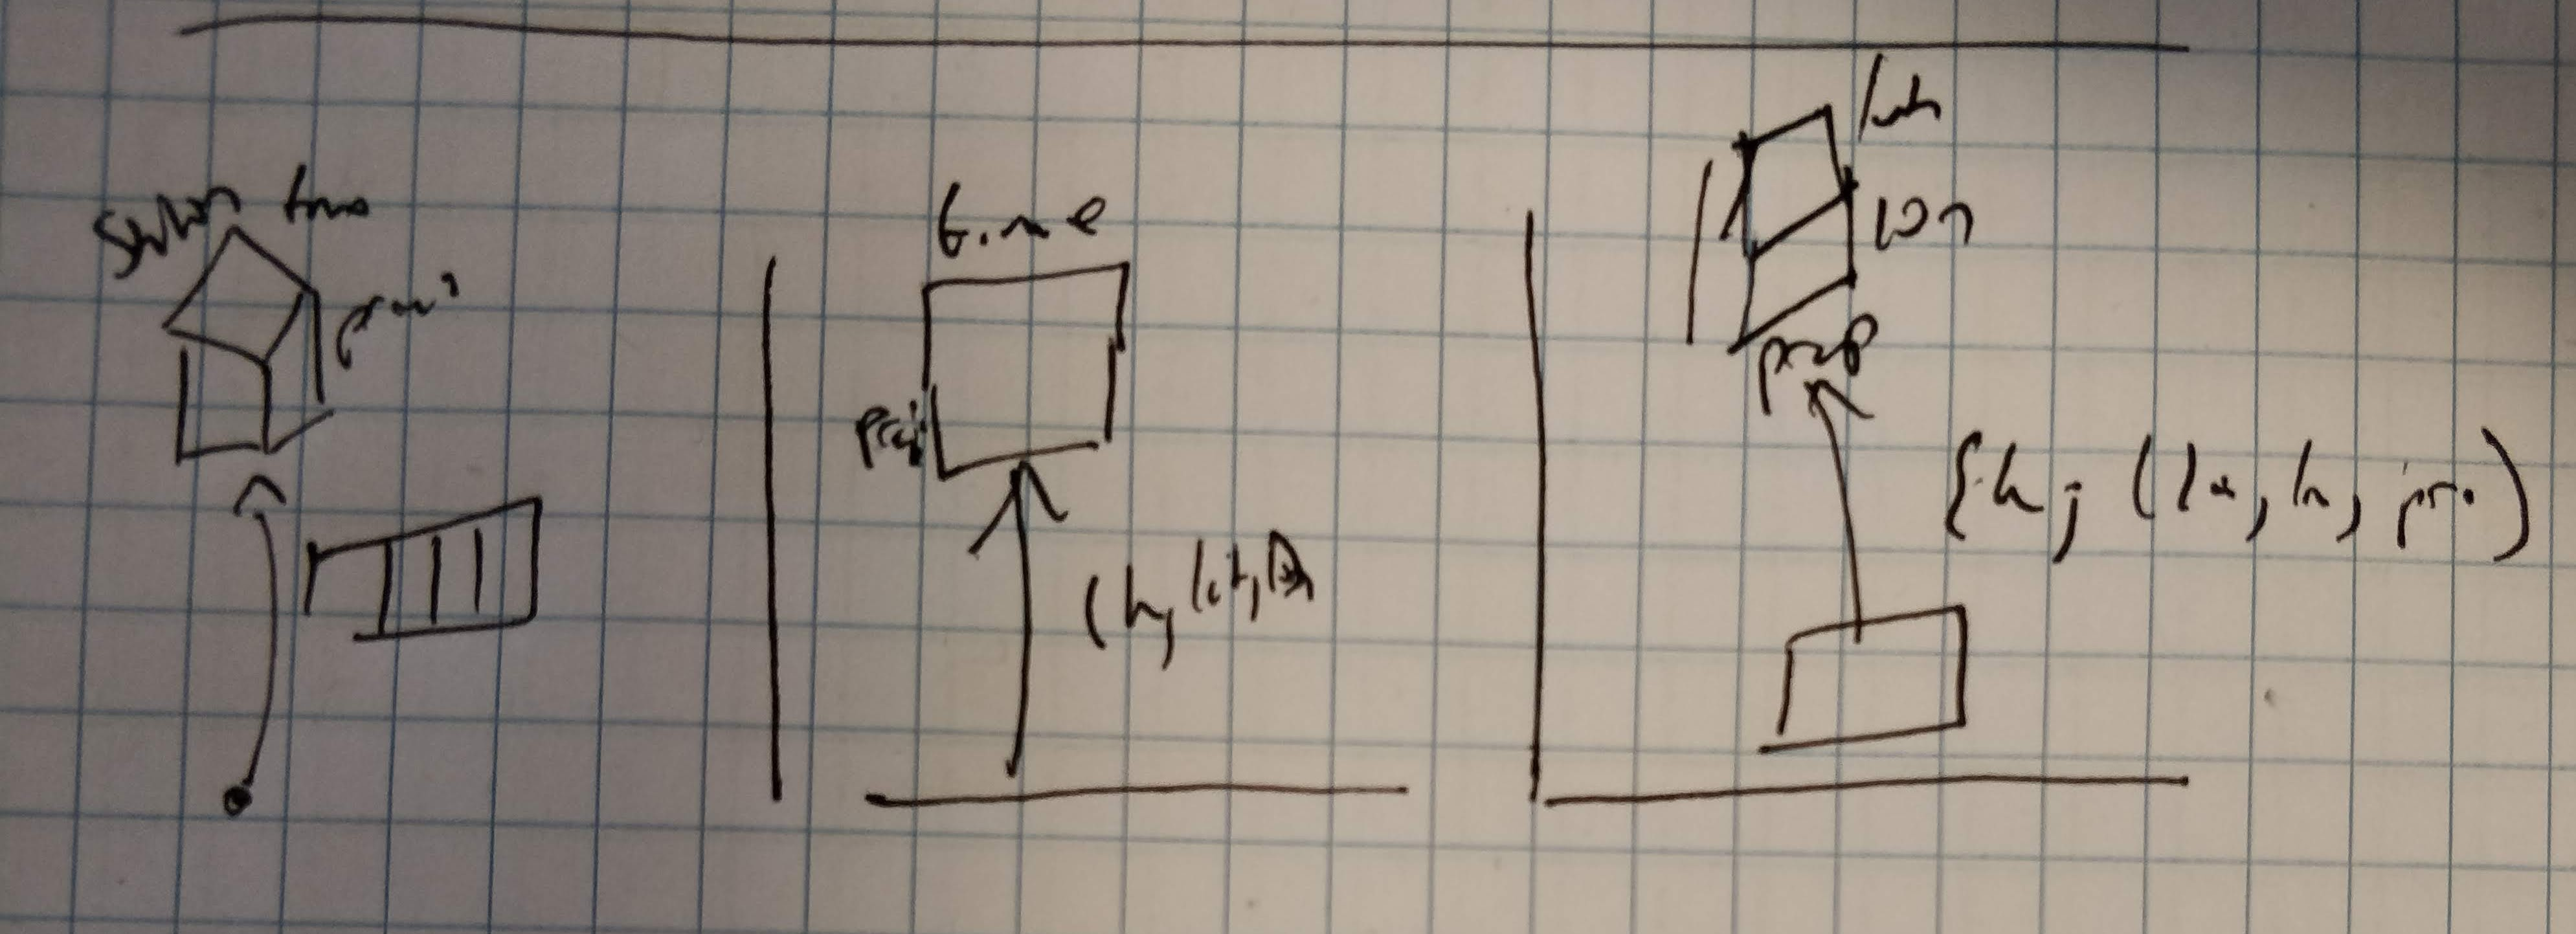
\includegraphics[width=\columnwidth]{dbundle.png}
  \caption{The table from \autoref{fig:related-work:continuity:ktypes} has a 3 dimensional fiber (name, temperature, precipitation), a 0D base space, and each row is a section. Each time series is a section of a bundle with a 2D fiber (time, precipitation) and a 1D base space encoding temporal continuity. Each location of the rain map is a section of a bundle with a 2D plane base encoding spatial continuity and a 3D fiber space encoding (latitude, longitude, precipitation)
    \label{fig:atct:trivialbundle}}
\end{figure}

In \autoref{fig:atct:trivialbundle}, the base space $\dbase$ acts as an indexing space into the fiber space $\dfiber$. In the bundle encoding of the table, the indexing space is arbitrarily numbered keys; in the time series bundle, the base space is the interval [0,1]; and the map is sparse samples from a continuous space $[0,1]^{2}$ In contrast to a notion of a semantic binding between indexing space and field values, as proposed by Munzner\cite{munznerVisualizationAnalysisDesign2014}, the fields describing the continuity are part of the fiber. For example, the time is a fiber in the time series and the latitude and longitude are part of the map's fiber. This separation between connectivity and what it is called means the time or location can change units without a change to structure. It also provides a way to express data that may seem continuous but isn't, for example independent measurements over time. The data in \autoref{fig:atct:trivialbundle} comes from the same dataset; therefore we know that the bundles share connectivity and fiber space. It is expected that shared components be translated to visual elements in a consistent manner \cite{hullmanKeeping2018}, and in \autoref{sec:artist:operators} we introduce operators for expressing which components are shared and how to verify that they have been mapped into visual elements in a consistent manner. 

\subsubsection{Uniform Abstract Graphic Representation}
One of the advantages of fiber bundles is that they are general enough that we can also encode the output of a visual algorithm as a bundle. This allows us to use the same structure to express the properties of data and the graphic that must be symmetric to the data in an equivariant (\autoref{sec:related-work:equivariance}) transformation. We denote the output as a graphic, but the use of bundles allows us to generalize to output on any display space, such as a screen or 3D print. 
\begin{equation}
  \label{eq:atct:fb:graphic}
  \begin{tikzcd}
      \gfiberc \arrow[r, hook, color=total] & \gtotalc \arrow[r, "\pi", two heads, color=total] & \gbasec
  \end{tikzcd}
\end{equation}
The total space \gtotalc\ is an abstraction of an ideal (infinite resolution) space into which the graphic can be rendered. The base space \gbasec\ is a parameterization of the display area, for example the inked bounding box in cairo \cite{CairographicsOrg}. The fiber space \gfiberc\ is an abstraction of the renderer fields; for example a 2 dimension screen has pixels that can be parameterized $ \gfiber=\{x,\,y\,z\,r,\,g,\,b,\,a\}$. 

As with data, we model the graphic generating functions as sections $\gsection$ of the graphic bundle 
\begin{equation}
  \label{eq:atct:fb_graphic_section}
  \cgamma{\opensetgc}{\gtotalc\restriction_{\opensetgc}} \coloneqq \big\{\gsectionc: \opensetgc\rightarrow \gtotalc\restriction_{\opensetgc} \; \bigm{\vert} \pi(\gsectionc(\gbasepointc)) = \gbasepointc\;for\, all\; \gbasepointc \in \opensetgc \big\}
\end{equation}
that map from a point in an openset in the graphic space $\gbasepoint \in \opensetg \subseteq \gbase$ to a point in the graphic fiber $\gfiber$. The section evaluated on a single point $\gbasepoint$ returns a single graphic record, for example one pixel in an ideal resolution space. In our model, the unevaluated graphic section is passed to a renderer to generate graphics. 

\begin{figure}[H]
  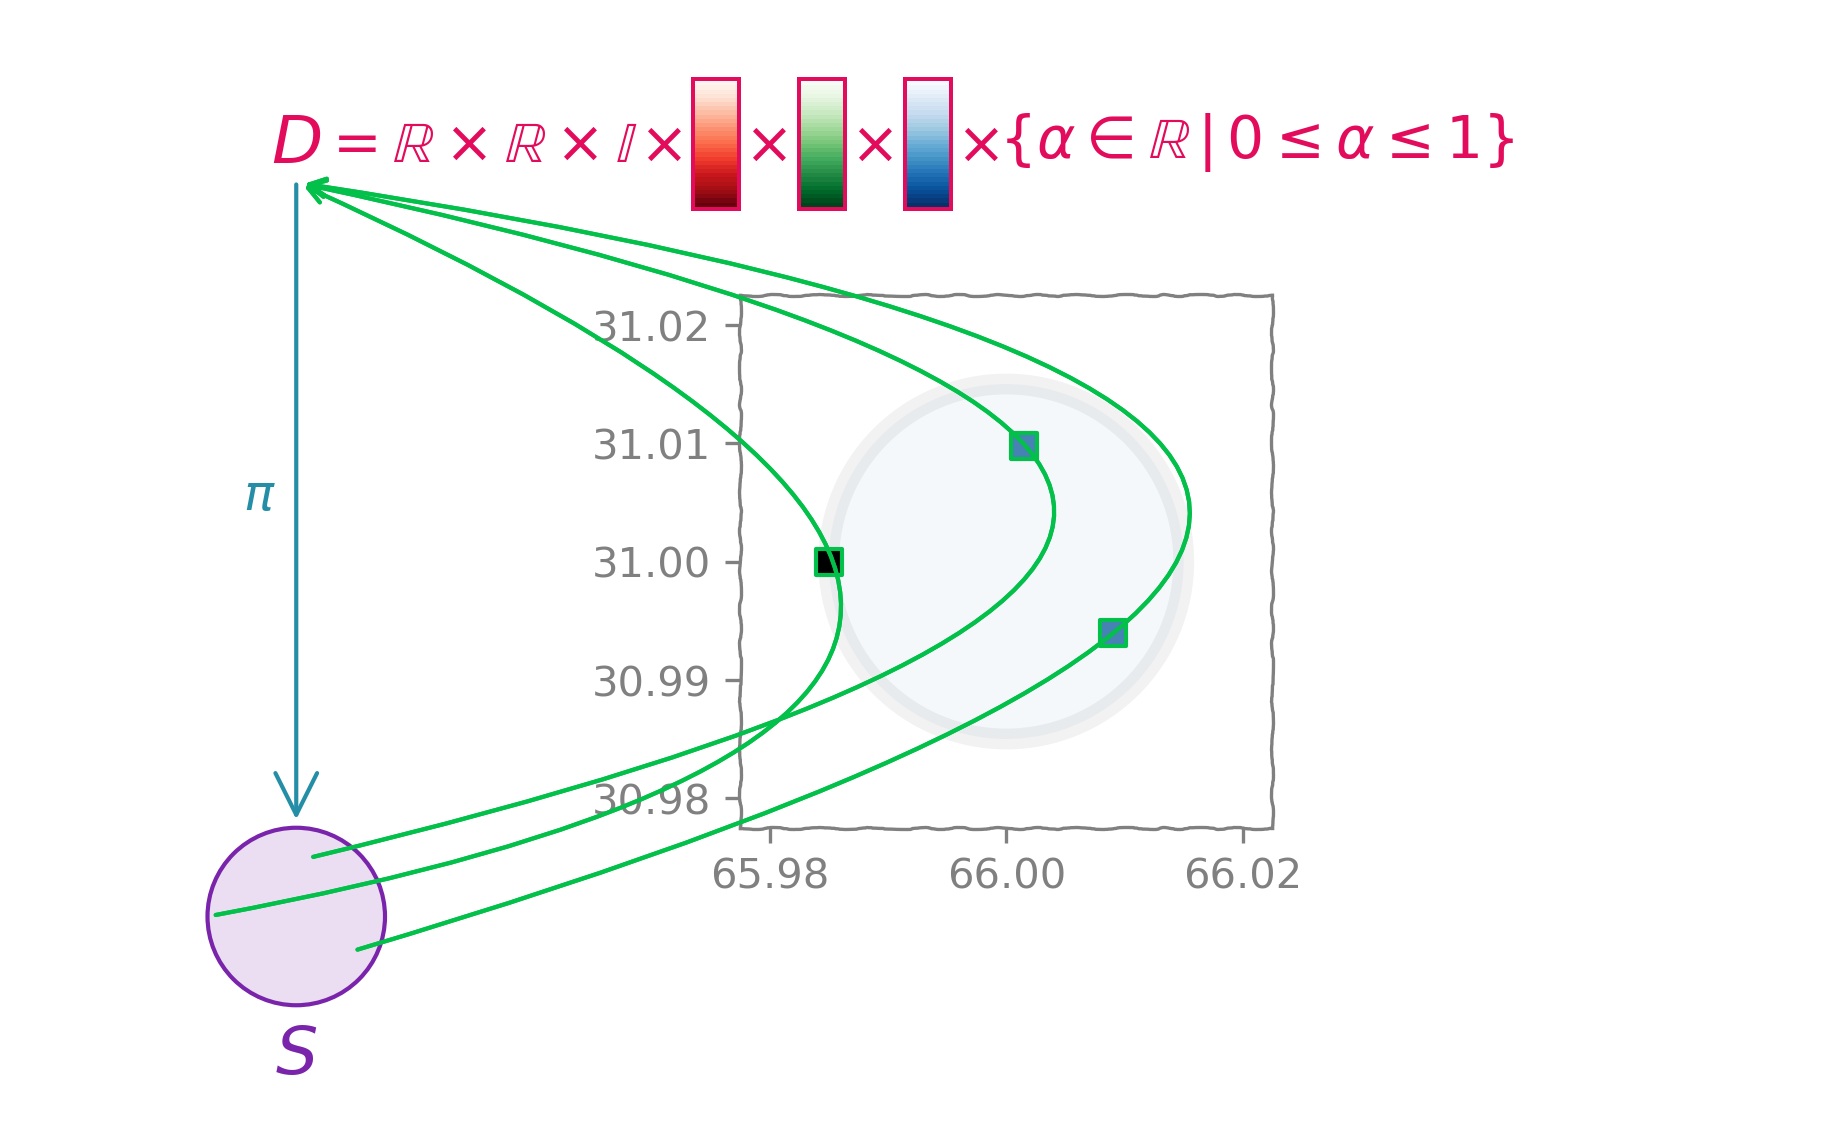
\includegraphics[width=1\columnwidth]{fb_rho.png}
  \caption{For a 2D display, a section $\gsection$ maps from each point $\gbasepoint$ into a fiber $\gfiber$ that encodes an RGB pre-render space with infinite resolution $\mathcal{R}^{2}$. Each tiny colored box is an approximation of the return value of the same section function $\gsection$ evaluated on different points $\gbasepoint \in \gbase$ in the base space. \note{add alpha and z channels and very faded out marker point} 
  \label{fig:atct:fb:graphic}}
\end{figure}

In \autoref{fig:atct:fb:graphic}, the section function $\gsection$ maps into the fiber for a simplified 2D RGB infinite resolution pre-render space and returns the $\{x,y,r,g,b\}$ values of a pixel in an infinite resolution space. In \autoref{fig:atct:fb:graphic} these pixels are approximated as the small orange and black colored boxes. Each pixel is the output of the $\gsection(\gbasepoint)$ section that intersects the box. The set of all pixels returned by a section evaluated on a given visual base space $\gsection|_{\gbase}$ can yield a visual element, such as a marker, line, or piece of a glyph. While \autoref{fig:atct:fb:graphic} illustrates a highly idealized space with no overlaps, overlaps can be managed via a fiber element $\gfiber_{z}$ for ordering. It is left to the renderer to choose how to blend layers based on $\gfiber_{z}$ and $\gfiber_{a}$. 

\subsection{Abstract Data Containers}
\label{sec:atct:sheaves}
While bundles provide a way to describe the structure of the data, sheaves are a mathematical way of describing the data container. Sheaves are an algebraic data structure that provides a way of abstractly discussing the bookkeeping that data containers must implement to keep track of the continuity of the data \cite{ghristElementaryAppliedTopology2014}. This abstraction facilitates representational invariance, as introduced by Kindlemann and Scheidegger\cite{kindlmannAlgebraicProcessVisualization2014}, since the container level is uniformly specified as satisfying sheaf constraints. These constraints generalize to data that is subset\note{one is not like the others}, distributed, streaming, and on-demand. 


We can mathematically encode that we expect data containers to preserve the underlying continuity of the indexing space and the mappings between indexing space and record space using a type of function called a functor. Functors are mappings between categories that preserve the domains, codomains, composition, and identities of the morphisms within the category\cite{riehlCategoryTheoryContext}.

\begin{definition}\cite{bradleyWhatFunctorDefinitions,bradleyTopologyCategoricalApproach2020} A \textbf{functor} is a map $F: \mathcal{C} \rightarrow \mathcal{D}$, which means it is a function between objects $F: \textbf{ob}(\mathcal{C}) \mapsto \textbf{ob}(\mathcal{D})$ and that for every morphism $f \in Hom(C_1, C_2)$  there is a corresponding function $F: Hom(C1, C2) \mapsto Hom(F(C_1), F( C_2))$.
A \textbf{functor} must satisfy the properties 
\begin{itemize}
  \item \textit{identity}: $F(id_{C}(C)) = id_{D}(F(C))$
  \item \textit{composition}: $F(g)\circ F(f) = F(g\circ f)$ for any composable morphisms $C_{1}\xrightarrow{f} C_2$, $C_2 \xrightarrow{g} C_3$ 
\end{itemize}
$F(C) \in \textbf{ob}(\mathcal{D})$ denotes the object to which an object $C$ is mapped, and $F(f) \in Hom(F_(C_1), F_(C_2))$ denotes the morphism that $f$ is mapped to. 
\end{definition}
Modeling the data container as a functor allows us state that, just like a functor, the container is a map between index space objects and sets of data records that preserve morphisms between index space objects and data records. 
\begin{equation}
  \label{eq:atct:sheaf:functor}
  \sheafc_{\dbasec, \dtotalc}: \opensetc \rightarrow \cgamma{\opensetc}{\dtotalc\restriction_{\opensetc}}
\end{equation}
A common way of encapsulating a map from a topological space to a category of sets is as a presheaf
\begin{definition}
  A \textbf{presheaf} $F:\mathcal{C}^{op} \rightarrow \setb$ is a contravariant functor from an object in an arbitrary category to an object in the category \setb\cite{nlab:presheaf, spanier1989algebraic}. 
\end{definition}
A functor is contravariant when the morphisms between the input objects go in the opposite direction from the morphisms between the output objects. The presheaf is contravariant because the inclusion morphisms between input objects 
\begin{equation*}
  \label{eq:atct:sheaf:inclusion}
  \iota: \opensetc_1 \rightarrow \opensetc_2
\end{equation*}
are defined such that they correspond to the partial ordering $\openset_1 \subseteq \openset_2$, but the restriction morphisms $\iota^*$ between the sets of sections 
\begin{equation*}
  \label{eq:atct:sheaf:restriction}
  \iota^*: \cgamma{\opensetc_2}{\dtotalc\restriction_{\opensetc_2}} \rightarrow \cgamma{\opensetc_1}{\dtotalc\restriction_{\openset_c1}}
\end{equation*}
restricts the larger set to the smaller one such that all functions that are continuous over a space must be continuous over a subspace $\Gamma_2 \subseteq \Gamma_1$, where $\Gamma_{i}\coloneqq\Gamma(\openset_{i}, \dtotal\restriction_{\openset_{i}})$. 


For example, lets define presheaves $\sheaf_1, \sheaf_2$. These are maps from intervals $\openset_1, \openset_2$ to a set of functions $\Gamma_1, \Gamma_2$ that are continuous over that interval: 
\note{Human readable before inline not after}

\begin{figure}[H]
  \includegraphics*[width=1\columnwidth]{figures/tex/presheaf.pdf}
  \caption*{presheafs $\sheaf_1, \sheaf_2$ mapping from intervals to the trignometric functions defined over those intervals }
\end{figure}

The constraints of a presheaf functor are that since the $constant, sin, cos$ functions are defined over the interval $\left[0,1\right]$, these functions must also be continuous over the sub-interval $\left(\frac{\pi}{2}, \frac{3\pi}{2}\right)$; therefore the sections in $\Gamma_{2}$ must also be included in the set of sections over the subspace $\Gamma_{1}$. The generalization of this constraint is that data structures that contain continuous functions must support interpolating them over arbitrarily small subspaces. 

While presheaves preserve the rules for sets of sections, sheaves add on conditions for gluing individual sections over subspaces into cohesive sections over the whole space. 
\begin{definition}\cite{bakerEuclideanSpaceMathsSheaf,spanier1989algebraic} A \textbf{sheaf} is a presheaf that satisfies the following two axioms
\begin{itemize}
  \item \textit{locality} two sections in a sheaf are equal $\dsection^{a} = \dsection^{b}$ when they evaluate to the same values over the same set of open sets $\dsection^{a}|_{\openset} =  \dsection^{b}|_{\openset}$.
  \item \textit{gluing} the union of sections defined on specific open sets is equivalent to one big section over the union of spaces $\dsection|_{\openset_{i} \cup \openset_{j}} = \dsection^{i}|_{\openset_i} \cup \dsection^{j}|_{\openset_j}$ if these sections agree on overlaps $\dsection^{i}|_{\openset_i\cap\openset_j} =  \dsection^{j}|_{\openset_i\cap\openset_j}$
  \end{itemize}
\end{definition}
The gluing axiom says that a distributed representation of a dataset, which is a set of local sections, is equivalent to a section over the union of the opensets of the local sections. The locality axiom asserts that the glued section function is equivalent to a function over the union if they evaluate to the same values. The gluing axiom can also be used to generate the gluing rules used to construct non-trivial bundles from the set of trivial local sections. Generally, the sheaf asserts the expectation that the data container is implemented such that the connectivity between the opensets (indexing subspaces) is preserved. 

Each section of a sheaf over a point returns a single record in the fiber. The sheaf over an open set $\openset$ surrounding a point $\dbasepoint$ is called a \textit{stalk}\cite{harder2008lectures}
\begin{equation}
  \label{eq:atct:sheaf:stalk}
    \sheaf_{\dbase, \dtotalc}\restriction_{\dbasepoint}\coloneqq \lim\limits_{\openset\ni \dbasepoint} \Gamma(\openset, \dtotal\restriction_{\openset}) 
\end{equation}
where the fiber is contained inside the stalk  $\dfiber_{\dbasepoint} \subset  \sheaf_{\dbase, \dtotal}\restriction_{\dbasepoint}$. The \textit{germ} is the section evaluated at a point in the stalk  $\dsection(\dbasepoint) \in \sheaf_{\dbase, \dtotal}\restriction_{\dbasepoint}$ and is the data. Since the stalk and the germ include the values near the limit of the point at \dbasepoint, the germ can be used to compute the mathematical derivative of the data for visualization tasks that require this information. 

\subsection{Data Index and Graphic Index Correspondence}
\label{sec:atct:xi}
There is an expectation that for a visualization to be readable, the visual elements must correspond to distinct data elements\cite{ziemkiewiczEmbeddingInformationVisualization2009} and we can use the properties of sheaves to formally express this correspondence. We first describe the relationship between the graphic indexing space \gbase\ and the data indexing space \dbase\, which we propose is one where multiple graphic indexes map to one data index, and every index in the graphic space can be mapped to an index in the data space. We encode these expectations as the \textcolor{functor}{map} \vindexc, which we define to be a surjective continuous map
\begin{equation}
  \label{eq:atct:xi}
  \vindexc: \opensetgc \textcolor{functor}{\rightarrow} \opensetc
\end{equation}
between a graphic subspace $\opensetg \subseteq \gbase$ and data subspace $\openset \subseteq \dbase$. The functor $\vindex$ is surjective 
such that we can identify the set of points in graphic space that correspond to each point in data space
\begin{equation}
  \label{eq:atct:xi:inverse}
  \vindexprec(\dbasepointc) = \{\gbasepointc | \vindexc(\gbasepointc) = \dbasepointc \forall \dbasepointc \in \dbase, \gbasepointc \in \gbasec\}
\end{equation}
and every point in a graphic space has a corresponding point in data space. 


We construct the map as going from graphic to data because that encodes the notion that every visual element traces back to the data in some way. As exemplified in \autoref{fig:atct:morphisms:sheaf}, we define $\vindex$ as a surjective map because it allows us to express that a union of graphic spaces $S_i$ maps to single data point $\dbasepoint$, which allows us to express visual representations of a single record that are the union of many primitives, such as multipart glyphs (e.g boxplots) and combinations of plot types (e.g line with point markers). 

\subsubsection{Data and Graphic Correspondence}
Since we have defined a function \vindex\ between two spaces $\dbase, \gbase$, we can then construct functors that transport sheaves over each space to the other\cite{harder2008lectures}. This allows us to describe what data we expect at each graphic index location and what graphic is expected at each data index location. Transport functors compose the indexing map \vindex\ with the sheave map to say that a record \dsection\ at \dbasepoint\ is at all corresponding \gbasepoint\ and that a function \gsection\ over one point \gbasepoint\ is the same function at all points $\gbasepoint \in \gbase$ that correspond to the same record index \dbasepoint.

\paragraph{\textbf{Graphic Corresponding to Data}}
The pushforward (direct image) sheaf establishes which graphic generating function $\gsection$ corresponds to a point $\dbasepoint \in dbase$ in the data base space.   
\begin{definition} Given a sheaf $\sheaf_{\gbase, \gtotal}$ on $\gbase$, the \textbf{pushforward} sheaf  $\vindexpush\sheaf_{\gbase, \gtotal}$ on $\dbase$ is defined as 
  \begin{equation*}
    \vindexpushc(\sheafc_{\gbasec, \gtotalc})(\opensetc)  = \sheafc_{\gbasec, \gtotalc}(\vindexc^{-1}(\opensetc))
  \end{equation*}
for all opensets $\opensetc \subset \dbasec$\cite{harder2008lectures}.
\end{definition}
The pushforward sheaf returns the set of graphic sections over the data base space that corresponds to the graphic space $\vindex^{-1}(\openset) = \opensetgc$. The pushforward functor $\vindexpushc$ transports sheaves of sections on $\opensetgc$ over $\openset$
 \begin{equation}  
  \cgamma{\opensetc}{\vindexpushc\gtotalc\restriction_{\opensetc}}  \ni \vindexpushc\gsectionc: \opensetc \rightarrow \vindexpushc \gtotalc\restriction_{\opensetc} 
\end{equation}
such that it provides a way to look up which graphic corresponds with a data index
\begin{equation}
  \vindexpushc\gsectionc(\dbasepointc) = \gsectionc\restriction_{\vindexprec(\dbasepointc)}
\end{equation}
such that $\vindexpush\gsection(\dbasepoint))(\gbasepoint) = \gsection(\gbasepoint)$ for all $\gbasepoint \in \vindexpre(\dbasepoint)$. Therefore, the continuous map $\vindex$ and transport functors $\vindexpull, \vindexpush$ allow us to express the correspondence between graphic section and data section.

\paragraph{\textbf{Data Corresponding to Graphic}}
The pullback (inverse image) sheaf establishes which data record  returned by $\dsection$ corresponds to a point $\gbasepoint \in \gbase$ in the graphic base space. 
\begin{definition} \cite{harder2008lectures} Given a sheaf $\sheaf_{\dbase, \dtotal}$ on $\dbase$, the \textbf{pullback} sheaf $\vindexpullc\sheafc_{\dbasec, \dtotalc}$ on $\gbasec$ is defined as the sheaf associated to the presheaf
  \begin{equation*}
    \vindexpullc(\sheafc_{\dbasec, \dtotalc})(\opensetgc) = \sheafc_{\dbasec, \dtotalc}(\vindexc(\opensetgc))   
  \end{equation*}
for $\vindex(\opensetgc) \in \dbase$.
\end{definition}
The pullback sheaf returns the set of data sections over the graphic base space that corresponds to the graphic space $\vindex(\opensetg) = \openset$. The pullback $\vindexpullc$ transports sheaves of sections on $\openset \subseteq \dbase$ over $\opensetg \subseteq \gbase$
\begin{equation}
  \cgamma{\opensetgc}{\vindexpullc\dtotalc\restriction_{\opensetgc}} \ni \vindexpullc\dsectionc: \opensetgc \rightarrow \vindexpullc \dtotalc\restriction_{\opensetgc}
\end{equation}
such that there is a way to then look up what data values correspond with a graphic index
\begin{equation}
  \vindexpullc\dsectionc(\gbasepointc) = \dsectionc(\vindexc(\gbasepointc)) = \dsectionc(\dbasepointc)
\end{equation}
As \vindex\ is surjective, there are many points $\gbasepoint \in \opensetg\subseteq\gbase$ in the graphic space that correspond to a single point $\vindex(\gbasepoint) = \dbasepoint$. 
 
\subsubsection{Example: Graphic and Data}
\begin{figure}[H]
  \includegraphics*[width=1\columnwidth]{xi_sin.png}
  \caption{The data consists of the $sin$ and $cos$ functions over a unit circle base space. We choose to visualize this as a circle and two line plots. The indexing function \vindex\ book keeps \note{find better word than bookkeeping} which parts of the circle and each curve correspond to each point on the unit circle. The pushforward $\vindexpush$ matches each point in the data space to the specification of the graphic at that point, while the pullback $\vindexpull$ matches each point in the graphic space to the data over that point. \label{fig:atct:morphisms:sheaf}} 
\end{figure}

Functors between sheaves are a way of expressing the bookkeeping involved in keeping track of which graphic section \gsection\ corresponds to which data section \dsection. The $(\dbasepoint_i, \gbase_i)$ pairing expressed in \autoref{eq:atct:xi} establishes that there is a correspondence between sections evaluated over $\dbasepoint_i$ and $\gbase_i$. This allows us to construct graphic specifications for each data index $\vindexpush\gsection$ and retrieve the data $\vindexpull\dsection$ for any graphic section generating any piece of a graphic. In \autoref{fig:atct:morphisms:sheaf}, the visualization is a graphic representation of a unit circle and the sin and cosine curves on that interval. The index lookup $\vindex$ describes which parts of the circle and curves are generated from which points on the unit circle. Given this correspondence, the pullback $\vindexpull\dsection$ looks up which values are being represented in a given part of the graphic. This type of lookup is critical for interactive techniques such as brushing, linking, and tooltips\cite{beckerBrushingScatterplots1987}. The pushforward $\vindexpush\gsection$ describes how a graphic is supposed to look for each point in the data space. The graphic parameterization in \autoref{fig:atct:morphisms:sheaf} is intended as an approximation of $\vindexpush\gsection$ and is akin to declarative visualization specs such as vega \cite{satyanarayanDeclarativeInteractionDesign2014} and svg \cite{quintScalable2003}. These specs and $\vindexpushc\gsection$ provide a renderer independent way of describing the graphic and are therefore useful for standardizing internal representation of the graphic and serializing the graphic for portability.  

\section{Codifying Structure Preservation}
\label{sec:artist}
In this work we propose that visualization libraries are implementing transformations from data sheaf to graphic sheaf. We call these subset of functions the artist:
\begin{align}
  \label{eq:artist:hom_transport}
  \vartistc:& \cgamma{\dbasec}{\dtotalc}\textcolor{artist}{\rightarrow} \cgamma{\gbasec}{\gtotalc}
\end{align}
 The artists can be constructed as morphisms of sheaves over the same base spaces through the application of pushforward and pullback functors; therefore they are natural transformations.
 \begin{definition} Given two functors $F,G$ with the same domain $\mathcal{C}$ and codomain $\mathcal{D}$, a \textbf{natural transformation} $\alpha: F \Rightarrow G$ is a map
\begin{itemize}
  \item \textit{data}: morphism $F(c) \xrightarrow{\alpha_{c}} G(c)$ for each object $c \in \mathcal{C}$
  \item \textit{property} when $f: c_1 \rightarrow c_2$ is a morphism in $\mathcal{C}$, the components of the natural transform commute $G(f) \circ \alpha_{c_1} = \alpha_{c_2} \circ F(f)$  
\end{itemize}
such that $\alpha = (\alpha_{c})_{c\in\mathcal{C}}$ is the set of all natural transformation components $\alpha_{c}$.\cite{bradleyWhatNaturalTransformation}
 \end{definition}
 This means that natural transforms are maps of functors that take the same input object and return objects in the same category\cite{milewskiCategoryTheoryProgrammers}. As illustrated in \autoref{eq:atct:sheaves:homset}, the sheaf functors
\begin{equation}
  \label{eq:artist:sheaf:base}
    \begin{tikzcd}
      \cgamma{\dbasec}{\dtotalc} &  & \dbasec \arrow[ll, "{\sheafc_{\dbasec, \dtotalc}}"', maps to, color=sheaf] \arrow[rr, "{\vindexpushc\sheafc_{\gbasec, \gtotalc}}", maps to, color=sheaf] &  & \cgamma{\dbase}{\vindexpushc\gtotalc} 
      \end{tikzcd}
\end{equation}
take as input an openset object \opensetc\ or \opensetgc\ and return sets of data and graphic sections that are objects in \setb. As a map between these sheaf functors, the artist has to preserve the $\iota, \iota^*$ morphisms of the presheaf functor, described in \autoref{eq:atct:sheaf:inclusion} and 
\autoref{eq:atct:sheaf:restriction}, such that the following diagram commutes:

\begin{equation}
  \label{eq:artist:natural_transform:inclusions}
  \begin{tikzcd}
    \dbasec_1 & \cgamma{\dbasec_1}{\dtotalc} 
    \arrow[dd, "\iota^*"', color=set] 
    \arrow[rr, "\vartistc_{\dbase_1}", color=artist] &  & 
    \cgamma{\dbasec_{1}}{\vindexpushc\gtotalc} 
    \arrow[dd, "\iota^*", color=set] \\
      &  &  &  \\
    \dbasec_{2} \arrow[uu, "\iota", hook, color=base] & 
    \cgamma{\dbasec_{2}}{\dtotalc} 
    \arrow[rr, "\vartistc_{\dbasec_2}", color=artist] &  & 
    \cgamma{\dbasec_{2}}{\vindexpushc\gtotalc}                      
    \end{tikzcd}
\end{equation}
 The diagram in \autoref{eq:artist:natural_transform:inclusions} shows that restricting a set of outputs of an artist to a set of graphic sections over a subspace is equivalent to restricting the inputs to data sections over the same subspace. Because the artist is a functor of sheaves, the artist is expected to translate the data continuity to graphic continuity such that the connectivity of subsets is preserved. This bookkeeping is necessary for any visualization technique that selectively acts on different pieces of a data set; for example streaming visualizations \cite{krstajicVisualizationStreamingData2013} and panning and zooming \cite{NekrasovskiEvaluationPanZoom2006}

The output of an artist \vartist\ is a restricted subset of graphic sections
\begin{equation}
  \label{eq:artist:output}
  \imartist{\gbasec}{\gtotalc} \coloneqq\\ 
  \{\gsectionc \mid\;\exists\;\dsectionc \in \cgamma{\dbasec}{\dtotalc}\;s.t.\; 
  \vartistc(\dsectionc) = \gsectionc,\; \vindexc(\gbasec) = \dbasec \}
\end{equation} 
that are, by definition, only reachable through a structure preserving artist, which we describe in \autoref{sec:artist:equivariant:artist}. We define this subset because the space of all sections $\cgamma{\opensetg}{\gtotal\restriction_{\openset}}$ includes sections that may not be structure preserving. For example, a section may go from every point in the graphic space to the same single point in the graphic fiber $\gsection(\gbasepoint_i) = d\; \forall \gbasepoint \in \gbase$ such that the visual output is a single inked pixel on a screen. 

\subsection{Homeomorphism}
As mentioned in \autoref{sec:related-work:continuity}, preserving the topology of a visualization means that each discrete piece of differentiable visual information corresponds to a distince element of the dataset\cite{ziemkiewiczEmbeddingInformationVisualization2009} in a way where the organization of elements is preserved. A generalization of this condition is the idea that the graphic space can be collapased into the data indexing space, which means that the data base space is a deformation retraction of the graphic base space\cite{hatcherAlgebraicTopology2002}. By defining the indexing look up function \vindex, introduced in \autoref{sec:atct:sheaves}, to be 
\begin{equation}
  \vindex: \dbase \times I \rightarrow \dbase s.t \vindex(\dbasepoint) = \dbasepoint \forall \dbasepoint \in \gbase
\end{equation}

we can assert that the data space \dbase acts as an indexing space into \gbase such that knowing the location on space yields the location on the other and any point in either base space or graphic space has a correspoinding point in the other space. 
\begin{figure}[H]
  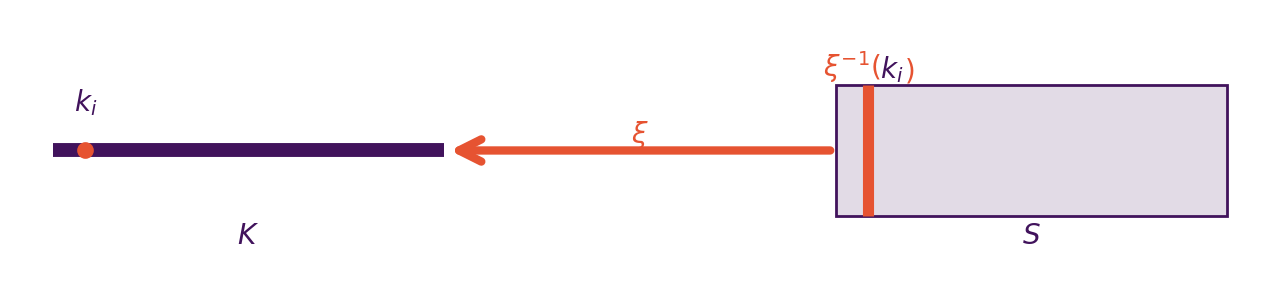
\includegraphics[width=1\columnwidth]{deform_retract.png}
  \caption{The graphic base space $\gbase$ is collapsible to the line $\dbase$ such that every band $(\dbasepoint_i, [0,1])$ on $\gbase$ maps to corresponding point $\dbasepoint_i \in \dbase$. The band $[0,1]$ determines the thickness of a rendered line for a given point $\dbasepoint_{i}$ by specifying how pixels corresponding to that point are colored. \label{fig:construction:xi}}
\end{figure}

For example, as shown in \autoref{fig:construction:xi}, a line is 1D but is a 2D glyph on a screen; therefore the graphic space $\gbase$ is constructed by multiplying the base space $\dbase$ with an interval $[0,1]$. Because $\gbase$ is collapsible into $\dbase$, every band $(\dbasepoint_i, [0,1])$ corresponds to a point in the base space $\dbasepoint_i \in \dbase$. The first coordinate $\alpha=\dbasepoint_i$ provides a lookup to retrieve the associated visual variables. The second coordinate, which is a point in the interval $\beta=[0,1]$. Together they are a point $\gbasepoint=(\alpha,\beta) \in gbase$ in the graphic base space. This point $\gbasepoint$ is the input into the graphic section $\gsection(\gbasepoint)$ that is used to determine which pixels are colored, which in turn determines the thickness, texture, and color of the line. 


\subsection{Equivariance}
\label{sec:artist:equiv}
As introduced in \autoref{sec:related-work:equivariance}, data and the corresponding visual encoding are expected to have compatible structure. This structure can be formally expressed as actions $\dfunc \in \dfuncset$ on the sheaf $\sheaf_{\dbase, \dtotal}$. We generalize from binary operations to a family of actions because that allows for expanding the set of allowable transformations on the data beyond a single operator. We describe the changes on the graphic side as changes in measurements \measure\, which are scaler or vector components of the rendered graphic that can be quantified, such as the color, position, shape, texture, or rotation angle of the graphic. The visual variables \cite{bertinIIPropertiesGraphic2011} are a subset of measurable components. For example, a measurement of a scatter marker could be its color (e.g. red) or its x position (e.g. 5). 

\subsubsection{Mathematical Structure of Data}
\label{sec:artist:equivariant:data}
\note{something something rotation etc}
We separate data transformations into two components, transformations on the base space $(\dfunchc, \dfuncpullc)$ and transformations on the fiber space $\dfunctc$. 

\begin{equation}
  \label{eq:artist:sheaves:monoid_morphism}
  \begin{tikzcd}
    \cgamma{\opensetc}{\dtotalc\restriction_{\opensetc}} 
    \arrow[rr, "\dfuncpullc", color=action, maps to] &  & 
    \cgamma{\opensetc^{\prime}}{\dfuncpullc\dtotalc\restriction_{\opensetc^{\prime}}} & 
    \cgamma{\opensetc^{\prime}}{\dfuncpullc\dtotalc\restriction_{\opensetc^{\prime}}} 
    \arrow[dd, "\dfunctc", color=action] \\
     &  & &       \\
    \opensetc 
    \arrow[uu, maps to,color=sheaf]  &  & \opensetc^{\prime} 
    \arrow[ll, "\dfunchc"', color=action, maps to] 
    \arrow[uu, maps to, color=sheaf] & \cgamma{\opensetc^{\prime}}{\dfuncpullc\dtotalc\restriction_{\opensetc^{\prime}}}                       
    \end{tikzcd}
\end{equation}
The base space transformation transforms one openset object $\openset^{\prime}$ to another object $\openset$, and the pullback functor transports the entire set of sections $\Gamma(\openset, \dtotal\restriction_{\openset})$ over the new base space $\Gamma(\openset^{\prime}, \dfuncpull\dtotal\restriction_{\openset^{\prime}})$. The fiber transformation transforms a single section $\dfuncpull\dsection$ to a different section $\dfuncpull\dsection$. 

\paragraph{\textbf{Topological structure}}
\noindent
The base space transformation is a point wise continuous map from one open set to another open set in the same base space
\begin{equation}
  \label{eq:atct:morphism:base}
 \dfunchc: \dbasepointc^{\prime}\mapsto \dbasepointc
 \end{equation}
such that $\openset, \openset^{\prime} \subseteq \dbase$. This means $\openset$ and $\openset^{\prime}$ are of the same topology type. To correctly align the sections with the remapped base space, there is a a corresponding section pullback function
\begin{equation}
  \label{eq:atct:morphism:basepull}
  \dfuncpullc \dsectionc \restriction_{\opensetc^{\prime}}: \dsectionc\restriction_{\opensetc^{\prime}} \mapsto \dsectionc \restriction_{\opensetc^{\prime} \circ \dfunchc} 
\end{equation}
such that $\dsection|_{\openset} = \dfuncpull\dsection|_{\opensetc^{\prime}}$ because $\dsection|_{\openset} = \dsection|_{\dfunch(\opensetc^{\prime})}$. This means that the base space transformation  $\dfunch(\dbasepoint^{\prime}) = \dfunch(\dbasepoint)$ such that  
\begin{equation}
  \label{eq:atct:morphism:verify_base}
  \dsectionc(\dbasec) = \dfuncpullc\dsectionc(\dbasepointc^{\prime}) = \dsectionc(\dfunchc(\dbasepointc^{\prime}))
\end{equation} 
which means that the index of the record changes from $\dbasepoint$ to $\dbasepoint^{\prime}$ but the values in the record are unmodified.

\paragraph{\textbf{Records}}
As introduced in \autoref{eq:artist:sheaves:monoid_morphism}, the fiber transformation $\dfunctc$ is a change in section 
\begin{equation}
  \label{eq:atct:morphism:fiber}
  \dfunctc: \dfuncpullc \dsectionc \restriction_{\opensetc^{\prime}} \mapsto \dfuncpullc \dsectionc^{\prime} \restriction_{\opensetc}
\end{equation}
where $\dsection, \dsection^{\prime} \in \Gamma(\openset^{\prime}, \dfuncpull\dtotal\restriction_{\openset^{\prime}})$. Since $\dfunct$ maps from one continuous function to another, it must itself be continuous such that
\begin{equation}
  \label{eq:atct:morphism:fiber:continuity}
   \lim\limits_{x \rightarrow \dbasepointc^{\prime}}\dfunctc(\dfuncpullc\dsectionc(x)) =  \dfunctc(\dfuncpullc\dsectionc(\dbasepointc^{\prime}))
\end{equation}
As mentioned in \autoref{sec:atct:fb:fiber}, $\dfunct$ is also  
a morphism on the fiber category $\dfunct \in Hom(\dfuncpull\dfiber\restriction_{\dbasepoint^{\prime}},\dfuncpull\dfiber\restriction_{\dbasepoint^{\prime}})$ restricted to a point $\dbasepoint^{\prime} \in \openset^{\prime}$. This means $\dfunct$ has to satisfy the properties of a morphism (\autoref{def:atct:category})
\begin{itemize}
  \item \textit{closed}: $\dfunctc(\dfuncpullc\dsectionc(\dbasepointc^{\prime})) \in \dfiberc$
  \item \textit{unitality}: $\dfunctc(id_{\dfiberc}(\dfuncpullc\dsectionc(\dbasepointc^{\prime}))) = id_{\dfiberc}(\dfunctc(\dfuncpullc\dsectionc(\dbasepointc^{\prime})))$
  \item \textit{composition and associativity}: \\
  $\dfunctc(\dfunctc(\dfuncpullc\dsectionc(\dbasepointc^{\prime}))) = (\dfunctc\circ\dfunctc)(\dfuncpullc\dsectionc(\dbasepointc^{\prime}))$
\end{itemize}

Additionally, $\dfunctc$ must preserve any features of $\dfiber$, such as operators that are defined as part of the structure of $\dfiber$. Examples of testing that $\dfunctc$ preserves the operations, and therefore structure, of the Steven's measurement scales are shown in \autoref{tab:appendix:summary:stevens}. We do not provide a general rule here because these constraints are defined with respect to how specific properties of the mathematical structure of individual fields $\dfiber$ are expected to be preserved rather than as a general consequence of $\dfunctc$ being a section map and morphism of the category. 

\paragraph{\textbf{Topological structure and records}} 
\noindent We define a full data transformation as one that induces both a remapping of the index space and a change in the data values
\begin{equation}
  \label{eq:atct:morphism:all}
  \dfuncc: \dsectionc\restriction_{\opensetc} \mapsto \dsectionc^{\prime}\restriction_{\opensetc} \circ \dfunchc
\end{equation}
which gives us an equation that can express transformations that have both a base space change and a fiber change. 

The data transform \dfunc\ is composable 
\begin{equation}
  \dfuncc = (\dfunchc, \prod\limits_{i=0}^{n}\dfunctc_i)
\end{equation}
if each (identical) component base space is transformed in the same way $\dfunch$ and there exists functions $\dfunc_{a,b}: \dtotal_a \times \dtotal_b \rightarrow \dtotal_a \times \dtotal_b$, $\dfunc_{a}: \dtotal_a \rightarrow \dtotal_a$ and $\dfunc_{b}: \dtotal_b \rightarrow \dtotal_b$ such that $\pi_a \circ \dfunc_a = \dfunc_{a,b} \circ \pi_a$ and $\pi_b \circ \dfunc_b = \dfunc_{a,b} \circ \pi_b$ then $\dfunc_{a,b} = (\dfunc_a, \dfunc_b)$. This allows us to define a data transform where each fiber transform $\dfunct_{i}$ can be applied to a different fiber field $\dfiber_i$. 

\begin{figure}[H]
  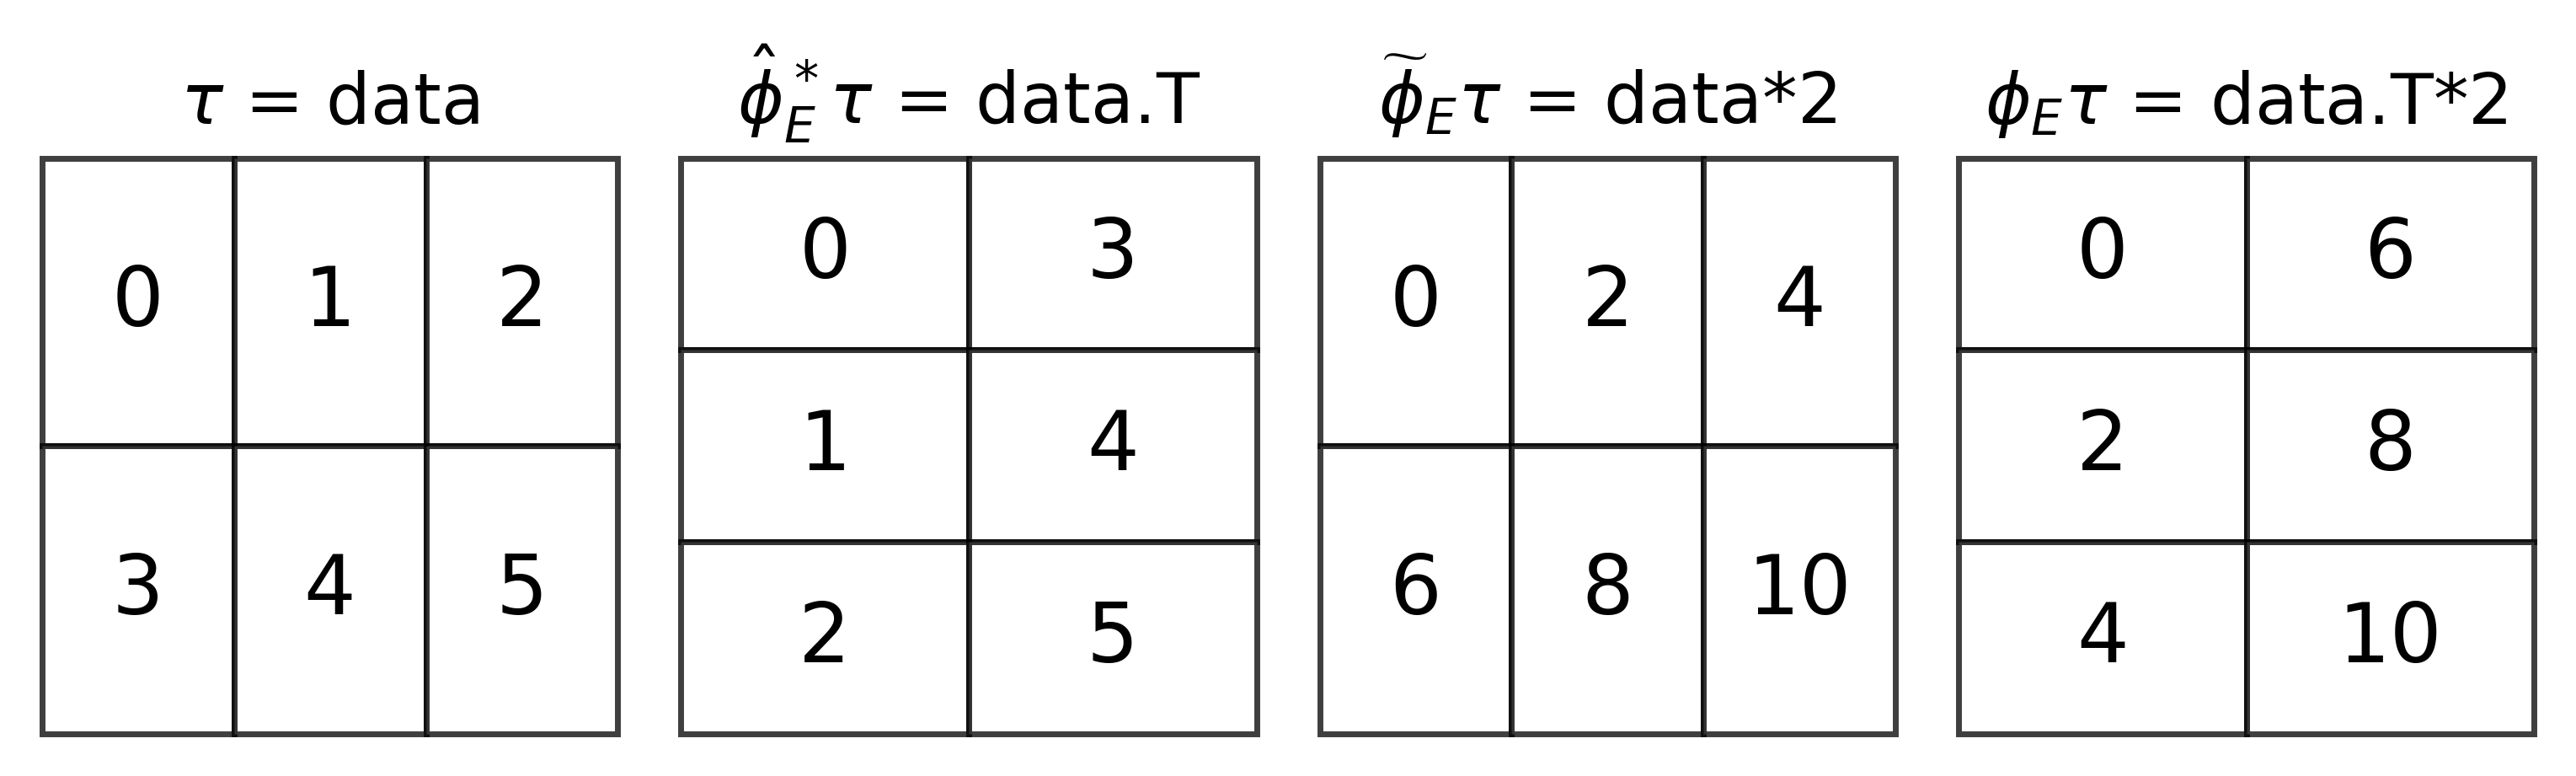
\includegraphics[width=\columnwidth]{phi.png}
  \caption{Values in a data set can be transformed in three ways: $\dfunch$-values can change position, .e.g transposed;  $\dfunct$-values can change, e.g. doubled; $\dfunc$ - values can change position and value  \label{fig:atct:phi}}
\end{figure}
\autoref{fig:atct:phi} provides an example of a transposition base space change \dfunch, a scaling fiber space change \dfunct, and a composition of the two \dfunc\ applied to each data point $x_{\dbasepoint} \in \texttt{data}$. In the transposition only case, the values in $\dfuncpull\dsection$ retain their neighbors from $\dsection$ because \dfunc\ does not change the continuity. Each value in $\dfuncpull\dsection$ is also the same as in $\dsection$, just moved to the new position. In $\dfunct\dsection$, each value is scaled by two but remains in the same location as in $\dsection$. And in $\dfunc\dsection$ each function is transposed such that it retains its neighbors and all values are scaled consistently.


\subsubsection{Equivariant Artist}
\label{sec:artist:equivariant:artist}
We formalize this structure preservation as equivariance, which is that for every morphism on the data $(\dfunch_{\dtotal}, \dfunct_{\dtotal})$ there is an equivalent morphism on the graphic  $(\dfunch_{\gtotal}, \dfunct_{\gtotal})$ The artist is an equivariant map if the diagram commutes for all points $\gbasepointc^{\prime}\in \gbasec^{\prime}$

\begin{equation}
  \label{eq:artist:equivariance}
  \begin{tikzcd}[ampersand replacement=\&, column sep=small]
  \cgamma{\dbasec}{\dtotalc} 
  \arrow[rrr, "\vartistc", color=artist] 
  \arrow[d, "\dfuncpullc_{\dtotalc}"', color=action] 
  \& \& \& 
  \imartist{\gbasec}{\gtotalc} 
  \arrow[d, "\dfuncpullc_{\gtotalc}", dotted] \\
  \cgamma{\dbasec^{\prime}}{\dfuncpullc_{\dtotalc}\dtotalc} 
  \arrow[dd, "\dfunctc_{\dtotalc}"', color=action] \& 
  \dbasec 
   \& 
  \gbasec 
  \arrow[l, "\vindexc"', color=functor] 
  \& 
  \imartist{\gbase^{\prime}}{\dfuncpullc_{\gtotalc}\gtotalc} 
  \arrow[dd, "\dfunctc_{\gtotalc}", dotted, color=action] \\
  \& 
  \dbasec^{\prime} 
  \arrow[u, "\dfunchc_{\dtotalc}", color=action] 
  \& 
  \gbasec^{\prime} 
  \arrow[l, "\vindexc"', color=functor] 
  \arrow[u, "\dfunchc_{\gtotalc}"', dotted, color=action] 
  \& \\
  \cgamma{\dbasec^{\prime}}{\dtotalc^{\prime}} 
  \arrow[rrr, "\vartistc", color=artist]  
  \& \& \& 
  \imartist{\gbasec^{\prime}}{\gtotalc^{\prime}}
  \end{tikzcd}
\end{equation}
such that starting at an arbitrary data point $\dsectionc(\dbasepointc)$ and transforming it into a different data point and then into a graphic 
\begin{equation*}
  \vartistc(\dfunctc_{\dtotalc}(\dsectionc(\dfunchc_{\dtotalc}(\vindexc(\gbasepointc^{\prime}))))) = \dfunctc_{\gtotalc}(\vartistc(\dsectionc(\vindexc(\dfunchc_{\gtotalc}(\gbasepointc^{\prime})))))
\end{equation*}
is equivalent to transforming the original data point into a graphic and then transforming the graphic into another graphic. The function $\dfunch_{\gtotal}$ induces a change in graphic generating function that matches the change in data. The graphic transformation $\dfunch_{\gtotal}$ is difficult to define because by definition it acts on a single record, for example a pixel in an idealized 2D screen.

Instead, we define an output \textcolor{action}{verification} function $\extractmc$ that takes as input the section evaluated on all the graphic space associated with a point $\gsection_{\vindexpre\restriction_{\dbasepoint}}$ and returns the corresponding \textcolor{action}{measurable visual components} $\measurec_{k}$. \note{formall define M as a space of measurements }
\begin{equation}
  \label{eq:artist:actual}
  \extractmc: (\gsectionc \circ \vindexpre) \mapsto (\dbasec \xrightarrow{\extractmc_{\gsectionc}} \measurec)
\end{equation}
The measurable elements can only be computed over the entire preimage because these aspects, such as thickness or marker shape, refer to the entire visual element. 
\begin{equation}
  \label{eq:artist:inout:diagram}
  \begin{tikzcd}[row sep=huge]
    \cgamma{\dbasec}{\dtotalc} 
    \arrow[rr, "\vartistc", color=artist] 
    \arrow[d, "\equivc"', color=monoid] &  & 
    \imartist{\gbasec}{\gtotalc} 
    \arrow[d, "render"] 
    \arrow[lld, "\extractmc"', color=monoid, dashed] \\
    {\textcolor{set}{Hom}(\dbasec, \measurec)}  &  & visualization 
    \arrow[ll, "measure",]
    \end{tikzcd}
\end{equation}
The extraction function is equivalent to measuring components of the rendered image $\extractm = measure\circ render$, which means an alternative way of implementing the function when $\gbase$ is not accessible is by decomposing the output into its measurable components.  

We also introduce a function \equivc\ that maps data to the measurement space directly 
\begin{equation}
\equivc: \dsectionc \mapsto (\dbase \xrightarrow{\equivc_{\dsectionc}} \measurec)
\end{equation}
such that $\equivc_{\dsection}(\dbasepointc)$ is the expected set of measurements $\measure_{\dbasepoint}$. The pair of \textcolor{monoid}{verification functions} (\equivc, \extractmc) can be used to test that the expected encoding $\equivb_{\dsection}$ of the data matches the actual encoding $\extractm_{\gsection}$ 
\begin{equation}
  \label{eq:artist:verification}
    \equivc(\dsectionc)(\dbasepointc) = \extractmc(\vartistc(\dsectionc))(\dbasepointc) = \extractmc(\gsectionc\circ\vindexprec)(\dbasepointc)=\measurec_{\dbasepointc}
\end{equation}

An artist is equivariant when changes to the input and output are equivariant. As introduced in \autoref{eq:atct:morphism:base}, the base space transformation \dfunch\ is invariant because $\dsection\restriction_{\openset} = \dsection\restriction_{\dfunch(\openset^{\prime})}$. This means that, for all points in the data $\dbasepoint \in \dbase$, the measurement should not change if only the base space is transformed 
\begin{equation}
  \label{eq:atct:equivarance:verify:base}
  \equivc(\dsectionc)(\dfunchc(\dbasepointc^{\prime})) = \extractmc(\vartistc(\dsectionc))(\dbasepointc)
\end{equation}
On the other hand, a change in sections \autoref{eq:atct:morphism:fiber} induces an equivalent change in measurements
\begin{equation}
  \label{eq:atct:equivarance:verify:fiber}
  \equivc(\dfunctc(\dsectionc))(\dbasepointc) = \dfunctc_{\measure}(\extractmc(\vartistc(\dsectionc))(\dbasepoint))
\end{equation}
The change in measurements $\dfunctc_{\measure}$ is defined by the developer as the symmetry between data and graphic that the artist is expected to preserve. 

\begin{figure}[H]
  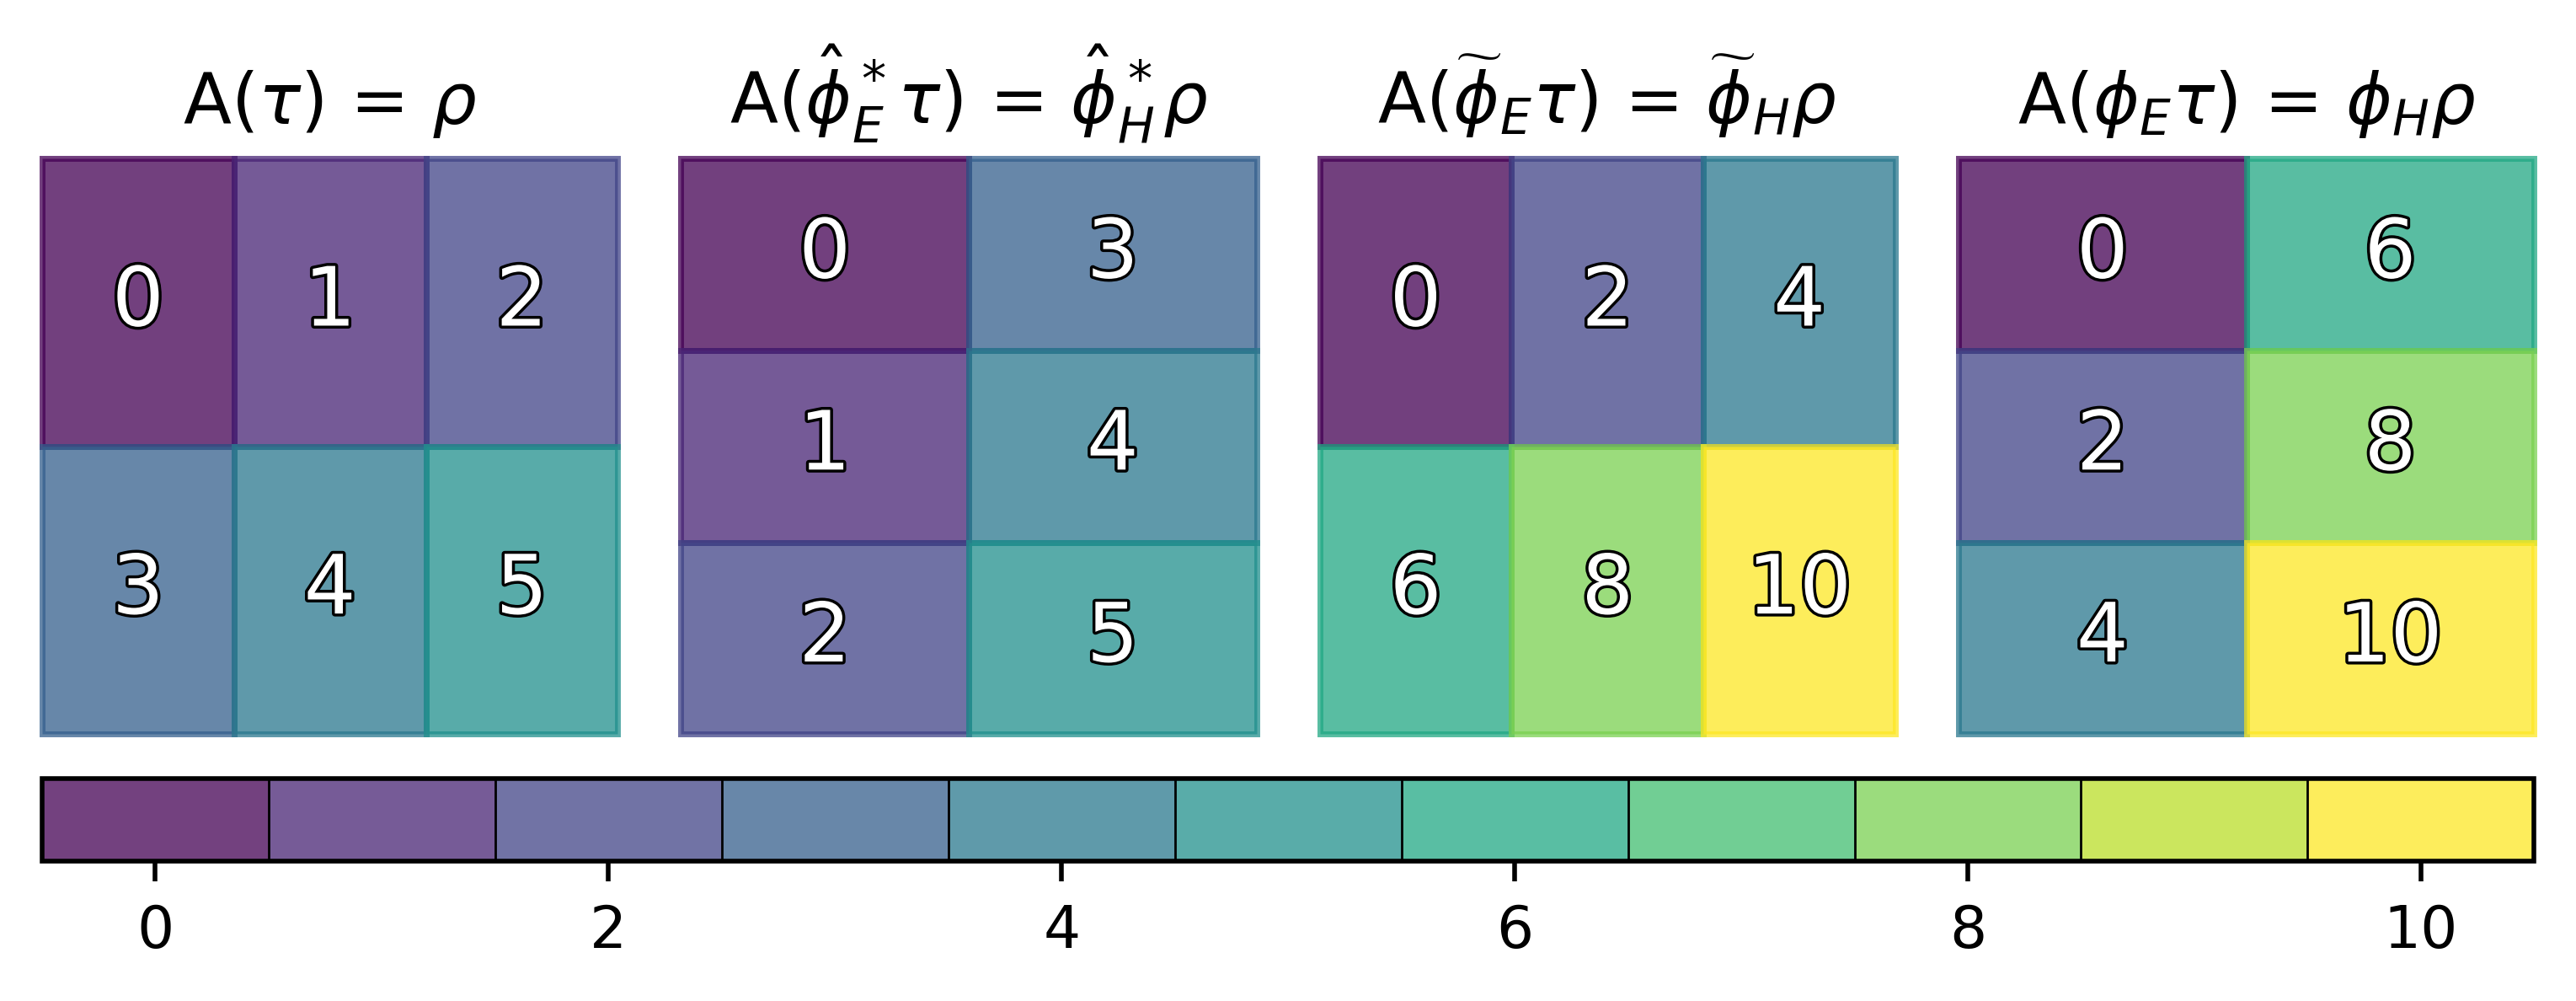
\includegraphics[width=1\columnwidth]{equivariance.png}
  \caption{This artist is equivariant because when the input data $\dsection$ is transposed, $\dfunch$, scaled $\dfunct$, and transposed and scaled $\dfunc$, the corresponding colored cells are transposed, scaled such that the color is moved two steps, and both transposed and scaled. 
  \label{fig:artist:equivariance}}
\end{figure}

For example, in \autoref{fig:artist:equivariance}, the measurable variable is color. This is a visual representation of the data shown in \autoref{fig:atct:phi}, and as such the equivariant transformations are an equivalent transposition and scaling of the colors. This visualization is equivariant with respect to base space transformations, as defined in \autoref{eq:atct:equivarance:verify:base}, because the color values at the new position at the old position $measure_\dbasepoint^{\prime} = \measure_{\dbasepoint}$. This visualization is also equivariant with respect to fiber wise transformations, as defined in \autoref{eq:atct:equivarance:verify:fiber}, because the colors are consistently scaled in the same was the data. For example, the values that have become 2 and 4 in the $\dfunctc$ and $\dfunc$ panels are colored the same as the original 2 and 4 values in the first panel. The equivariance in this visualization is composable, as shown in the colors being both transposed and scaled correctly in the $\dfunc$ panel.

\subsection{Composing Artists}\label{sec:artist:operators}
\note{addition: intersections mapped same, multiplication: fibers mapped same}
\note{large big data glued together correctly}
A common use of category theory in software engineering is the specification of modular components \cite{wielsManagementEvolvingSpecifications1998} such that we can build systems where the structure preserved by components is preserved in the composition of the components. This allows us to express that an artist that works on a dataset can be composed of artists that work on sub parts of that dataset. 


\subsubsection{Addition}
\label{sec:artist:addition}
We propose an addition operator that states that an artist that takes in a dataset can be constructed using artists that take as inputs subsets of the dataset

\begin{equation*}
  \label{eq:artist:addition}
  \vartistc_{a+b}(\cgamma{\dbasec^{a} \sqcup_{\dbase^c} \dbasec^b}{\dtotalc}) \coloneqq \vartistc_{a}(\cgamma{\dbasec^{a}}{\dtotalc}) + \vartistc_{b}(\cgamma{\dbasec^{b}}{\dtotalc}) 
\end{equation*}
As introduce in $\autoref{eq:artist:hom_transport}$, the artist returns a function $\gsection$. We assume that the output space is a trivial bundle, which means that $\gsectionc \in Hom(\gbase, \gfiber)$ because the output specification is the same at each point $\gbase$. This allows us to make use of the hom set adjoint property\note{find citation}\
\begin{equation*}
  Hom(\gbase^{a} + \gbasec^b, \gfiber) = Hom(\gbase^{a}, \gfiber) + Hom(\gbase^b, \gfiber)
\end{equation*} 
to define an artist constructed via addition as consisting of two distinct graphic sections
\begin{equation}
  \label{eq:artist:plus:output}
  \gsectionc(\gbasepointc) \coloneqq \begin{cases} \gsectionc^{a}(\gbasepointc) & \gbasepointc \in \vindexprec(\dbasec^{a}) \\
    \gsectionc^{b}(\gbasepointc) & \gbasepointc \in \vindexprec(\dbasec^{b})
  \end{cases}
\end{equation}
that are evaluated only if the input graphic point is an the graphic area that graphic section acts on. 

One way to verify that these artists are composable is to check that the return the same graphic on points in the intersection $\dbase^{c}$.  Given $\dbasepointc_{a} \in \dbasec_{c} \subset \dbasec_{a}$ and $\dbasepointc_{b} \in \dbasec_{c} \subset \dbasec_{b}$, if $\dbasepointc_{a} = \dbasepointc_{b}$ then

\begin{equation}
  \label{eq:artist:plus:verify}
  \begin{split}
  &\vartistc_{a+b}(\dsectionc^{a+b}(\dbasepointc_{a})) \\ 
  & = \vartistc_{a}(\dsectionc^{a}(\dbasepointc_{a})) = \vartistc_{b}(\dsectionc^{b}(\dbasepointc_{b}))
  \end{split}
\end{equation}
 for all $\dbasepointc_{a}, \dbasepointc_{b} \in \dbasec_{a}\bigsqcup\limits_{\dbasec_{c}} \dbasec_{b}$  
 
 \note{replace w/ a line plot w/markers}
 One example of an artist that is a sum of artists is a sphere drawer that draws different quadrants of a sphere $\vartist(\dsection) = \vartist_{1}(\dsection_{1}) + \vartist_{2}(\dsection_{2}) + \vartist_{3}(\dsection_{3}) \vartist_{4}(\dsection_{4})$. Given an input $\dbasepoint \in \dbase_4$ in the 4th quadrant, then the graphic section that would be executed is $\gsection_{4}$. If that point is also in the 3rd quadrant  $\dbasepoint \in \dbase_3$, then both artist outputs must return the same values $\gsection_{4}(\vindexprec(\dbasepoint)) = \gsection_{3}(\vindexprec(\dbasepoint))$. 


\subsubsection{Multiplication}
\label{sec:artist:operator:multiplication}
\note{fiber product vs cartesian product}

In the trivial case where the base spaces are the same $\dbase^{a} = \dbase^{b} = \dbase$, this is equivalent to adding more fields to a dataset. 

\begin{equation*}
  \label{eq:artist:multiplication}
  \vartistc_{a \times b}(\cgamma{\dbase}{\dtotalc^{a\times b}}) \coloneqq \vartistc_{a}(\cgamma{\dbasec}{\dtotalc^{a}}) \times \vartistc_{b}(\cgamma{\dbasec}{\dtotalc^{b}}) 
\end{equation*}

which following from an adjoint property of homsets \note{find citation and push this into a footnote or appendix maybe} 
\begin{equation}
  Hom(\gbase, \gfiber) \times Hom(\gbase, \gfiber) = Hom(\gbase, \gfiber\times \gfiber)
\end{equation}

which means that the artists on the subsets of fibers can be defined 
\begin{equation}
  \gsectionc^{a \times b} = \{\gsectionc^{a}(\gbasepointc), \gsectionc^{b}(\gbasepointc)\}, \gbasepointc \in \vindexprec(\dbasec)
\end{equation} 
but that the signature of $\gsectionc^{a \times b}$ would be $\gbase \rightarrow \gfiber \times \gfiber$. Instead of having to special case the return type of artists that are compositions of multiple case, the hom adjoint \note{find cite} property
\begin{equation*}
  Hom(\gbase, \gfiber \times \gfiber) = Hom(\gbase+\gbase, \gfiber)
\end{equation*}
 means that multiplication can be considered as a special case of addition where $\dbase^{a} = \dbase^{b}$. While we discussed the trivial case in \autoref{sec:artist:addition}, there is no strict  requirement that $\dfiber^{a} = \dfiber^{b}$. 

One way to verify that these artists are composable is to check that they encode any shared fiber $\dfiber^{c}$ in the same way.

\begin{equation}
  \begin{split}
    &\extractmc(\vartistc_{a\times b}(\dsectionc^{a\times b}(\dbasepointc)))\restriction_{\dfiberc^{c}}\\ 
    &= 
    \extractmc(\vartistc_{a}(\dsectionc^{a}(\dbasepointc_{a})))\restriction_{\dfiberc^{c}} = \extractmc(\vartistc_{b}(\dsectionc^{b}(\dbasepointc_{b})))\restriction_{\dfiberc^{c}}
  \end{split}
\end{equation}

This expectation of using the same encoding for the same variable is a generalization of the concept of consistency checking of multiple view encodings discussed by Qu and Hullman \cite{hullmanKeeping2018}. This expectation can also be used to check that a multipart glyph is assembled correctly. For example, a box plot \cite{wickham40YearsBoxplots2011} typically consists of a rectangle, multiple lines, and scatter points; therefore a boxplot artist $\vartist_{boxplot} = \vartist_{rect} \times \vartist_{errors} \times \vartist_{line} \times \vartist_{points}$ must be constructed such that all the sub artists draw a graphic at or around the same x value. 

\begin{figure}[H]
  \centering
  \includegraphics*[scale=.75]{qcom.png}
  \caption{The circle-line visual element can be constructed via $\gsection_{circle}$ + $\gsection_{line}$ functions that generate the circle and line elements respectively. This is equivalent to a $\gsection_{circle+line}$ function that takes as input the combined base space $\gbase_{circle} \sqcup \gbase_{line} = \gbase_{circle-line}$ and returns pixels in the circle-line element.  \label{fig:artist:operator}}
\end{figure}
There is no way to visually determine whether a visual element is the output of a single artist or a multiplied or added collection of artists. The circle-line visual element in \autoref{fig:artist:operator} can be a visual representation of a highlighted point intersecting with a line plot with the same fields. The same element can also be encoding some fields of a section in the circle and other fields of that section in the lines. \note{+*equive}
Although we have been discussing the trivial cases of adding observations or adding fields, this merging of artists in datasets can be generalized:
\begin{equation}
  \label{eq:artist:join_base_fiber}
  \vartistc(\cgamma{\mathop{\sqcup}_{i} \dbasec^{i}}{\mathop{\oplus}_{i}\dtotalc^{i}}) \coloneqq \sum_{i}
  \vartistc_{i}(\cgamma{\dbasec^{i}}{\dtotalc^{i}}) 
\end{equation} 

As shown in \autoref{eq:artist:join_base_fiber}, bundles over a union of base spaces can be joined as a product of the fibers. This allows us to consider all the data inputs in a complex visualization as a combined input, where some sections evaluate to null in fields for which there are no values for that point in the combined base space $\dbasepoint \in \mathop{\sqcup}_{i} \dbase^{i}$ The combined construction of the data is a method for expressing what each data input has in common with another data input-for example the data for labeling tick marks or legends- 
and therefore which commonalities need to be preserved in the artists that act on these inputs. 

\section{Constructing Structure Preserving Components}
\label{sec:construction}
\note{add a high level diagram Data->V->Screen}
\note{add back in path of Q, use tikz backend to convert to pgf to then tweak}
We propose that one way of constructing artist functions is to separate generating a visualization into an encoding stage $\vchannelc$ and a compositing stage $\vmarkc$. In the \textcolor{artist}{encoding} stage $\vchannelc$, a data bundle is treated as separable fields and each field is mapped to a measurable visual variable. In the encoding stage, many of the expected visual mappings $\equivb$ can be implemented inside the library. Factoring out the encoding stage leaves the \textcolor{artist}{compositing} stage $\vmarkc$ responsible for faithfully translating those measurable visual components into a visual element.  

As mentioned in \autoref{sec:artist:homeomorphic}, we construct the data base space as a deformation retraction of the graphic space. On simple way of doing so is to construct the graphic base space as a constant multiple of the base space such that 
\begin{equation}
  \underbrace{\dbasec\times[0,1]^{n}}_{\gbasec} \textcolor{functor}{\xmapsto{\hspace{1em}\vindexc\hspace{1em}}} \dbasec
\end{equation}
where n is a thickening of the graphic base space $\gbase$ to account for the dimensionality of the output space
\begin{equation*}
  n = \begin{cases}
    dim(\gbase) - dim(\dbase) & dim(\dbase)<dim(\gbase)\\
  0 & otherwise
  \end{cases}
\end{equation*}
because otherwise the data dimensionality $\dbase$ may be too small for a graphic representation. For example, as shown in \autoref{fig:construction:xi}, a line is 1D but is a 2D glyph on a screen; therefore the graphic space $\gbase$ is constructed by multiplying the base space $\dbase$ with an interval $[0,1]$. 

\subsection{Measurable Visual Components}
\label{sec:construction:vtotal}
We encapsulate the space of measurable components reachable through the encoding stage $\vchannel$ as a visual fiber bundle $\vfiberc \hookrightarrow \vtotalc \xrightarrow{\pi} \dbasec$. The  restricted fiber space $\vfiber$ of the bundle acts as the specification of the internal library representation of the measurable visual components. The space of visual sections $\cgamma{\opensetc}{\vtotalc\restriction_{\opensetc}} \coloneqq \big\{\vsectionc: \opensetc\rightarrow \vtotalc\restriction_{\opensetc} \; \bigm{\vert} \pi(\vsectionc(\dbasepointc)) = \dbasepointc\;for\, all\; \dbasepointc \in \opensetc \big\}$ return a visual encoding $\vsectionc(\dbasepoint)$ corresponding to data record $\dbasepoint(\dbasepoint)$.  Since the data bundle $dtotal$ and visual bundle $\vtotal$ have the same continuity $\pi(\dsection(\dbasepoint)) = \pi(\vsection(\dbasepoint))$, they are considered structurally equivalent such that $\dtotal=\vtotal$. The distinguishing characteristic of $\vtotal$ is that it is part of the construction of the artist and therefore a part of the visualization library implementation. We propose that reusing the fibers $\vfiber$ across components facilitates standardizing internal types across the library and that this standardization improves maintainability (\autoref{tab:appendix:library_spec}). 


\subsection{Component Encoders}
\label{sec:construction:nu}

As introduced in \autoref{sec:artist:equiv}, there is a set $\equivb$ of functions that map between data and corresponding visual encodings. We propose that for visualization library components to be structure preserving, they must implement a constrained subset of these encoding functions 
\begin{equation}
\cgamma{\dbasec}{\dtotalc} \xrightarrow{\vchannelc} \cgamma{\dbasec}{\vtotalc}  \subset \cgamma{\dbasec}{\dtotalc} \xrightarrow{\equivc}\textcolor{set}{Hom}(\dbasec, \measurec)
\end{equation}
that preserve the categorical structure (operators and morphisms) of the fiber and the continuity of the data section. As mentioned in \autoref{sec:construction:vtotal}, the total visual space is restricted to the space of data types internal to the library $\vfiber \subset \measure$ and sections are subsets of homsets $\Gamma(\dbase, \vtotal) \subset Hom(\dbase, \measure)$ because sections must be continuous.

The encoding functions $\vchannel$ are fiber wise transforms such that $\pi(\dtotal) = \pi(\vchannel(\dtotal))$. A consequence of this property is that $\vchannelc$ can be constructed as a point wise transformation such that  
\begin{equation}
  \label{eq:constrution:nu}
  \vchannelc: \dfiberc_{\dbasepointc} \rightarrow \vfiberc_{\dbasepoint}
\end{equation}
which means that means that a point in a single data fiber $\delement \in \dfiber_{\dbasepointc}$ can be mapped into a corresponding point in a visual fiber $\velement \in \vfiber_{\dbasepointc}$. This means that an encoding function $\vchannel$ can convert a single record independent of the whole dataset. 

Since $\dtotal$ and $vtotal$ are structurally identical, any $\vtotal$ can be redefined as $\dtotal$; therefore, as shown in \autoref{eq:construction:nu:fabrication}, any collection of $\vchannel$ functions can be composed such that they are equivalent to a $\vchannel$ that directly converts the input to the output.
\begin{equation}
  \label{eq:construction:nu:fabrication}
  \begin{tikzcd}
    \dfiberc_{\dbasepointc} 
    \arrow[rr, "\vchannelc", color=artist] 
    \arrow[rrrr, "\vchannelc^{\prime\prime}", dashed, bend right, color=artist] &  & 
    \vfiberc_{\dbasepointc}\coloneqq{\dfiberc_{\dbasepointc}^{\prime}} 
    \arrow[rr, "\vchannelc^{\prime}", color=artist] &  & 
    \vfiberc^{\prime}_{\dbasepointc}
  \end{tikzcd}
\end{equation}
 As with artists, $\vchannel$ are maps of sections such that the operators defined in \autoref{sec:artist:operators} can also act on transformers $\vchannel$, meaning that encoders can be added $\vchannel_{a+b} = \vchannel_{a} + \vchannel_{b}$ and multiplied d $\vchannel_{a\times b} = \vchannel_{a}  \vchannel_{b}$.  Encoders designed to satisfy these composability constraints provide for a rich set of building blocks for implementing complex encoders.

\subsubsection{Encoder Verification}
\label{sec:construction:nu:verification}
A  motivation for constructing an artist with an encoder stage $\vchannel$ is so that the conversion from data to measurable component can be tested separately from the assembly of components into a glyph. 
\begin{equation}
  \label{eq:construction:nu:validate}
  \begin{tikzcd}[column sep=4em]
    {\dfiberc_{\dbasepointc}^{a}} \times {\dfiberc_{\dbasepointc}^{b}} 
    \arrow[d, "\pi_a"', color=fiber] 
    \arrow[r, "\vchannelc_{ab}", color=artist] 
    \arrow[rr, "\equivc_{ab}", bend left, color=monoid]  & 
    {\vfiberc_{\dbasepointc}^{a}} \times {\vfiberc_{\dbasepointc}^{b}} 
    \arrow[d, "\pi_a", color=fiber] & 
    \measurec_{\dbasepointc}^{ab} 
    \arrow[d, "\measurec\restriction_a", color=set] \\
    \dfiberc_{\dbasepointc}^a 
    \arrow[r, "\vchannelc_{a}", dashed, color=artist] & 
    \vfiberc_{\dbasepointc}^a 
    \arrow[r, "\simeq", dotted]  & 
    \measurec_{\dbasepointc}^a   \\
    {\dfiberc_{\dbasepointc}^{a}} \times {\dfiberc_{\dbasepointc}^{c}} 
    \arrow[u, "\pi_a", color=fiber] 
    \arrow[r, "\vchannelc_{ac}", color=artist] 
    \arrow[rr, "\equivc_{ac}", bend right, color=monoid] & 
    {\vfiberc_{\dbasepointc}^{a}} \times {\vfiberc_{\dbasepointc}^{c}} 
    \arrow[u, "\pi_a"', color=fiber] & 
    \measurec_{\dbasepointc}^{ac} 
    \arrow[u, "\measurec\restriction_a"', color=set]            
    \end{tikzcd}
\end{equation}
As shown in \autoref{eq:construction:nu:validate}, an encoder is considered valid if there is an isomorphism between the actual outputted visual component and the expected measurable component encoding. An encoder is consistent if it encodes the same field in the same way even if coming from different data sources. 

An encoding function $\vchannelc$ is equivariant if the change in data, as defined in \autoref{sec:artist:equivariant:data}, and change in visual components are equivariant. Since $\dtotal$ and $\vtotal$ are over the same base space and are point wise, the base space change $\dfunch_{\dtotal}$ applies to both sides of the equation 
\begin{equation}
  \vchannelc(\dsectionc_{\dtotalc}(\dfunchc_{\dbasec}(\dbasepointc^{\prime}))) = \vsectionc(\dfunchc_{\dbasec}(\dbasepointc^{\prime}))
\end{equation}
and therefore there should not be a change in encoding. On the other hand, a change in the data values $\dfunct_{\dtotal}$ must have an equivalent change in visual components
\begin{equation}
  \dfunctc_{\vtotalc} \vchannelc(\dsectionc(\dbasepoint)) = \vchannelc(\dfunctc_{\dtotalc}(\dsectionc(\dbasepointc)))
\end{equation}
The change in visual components $\dfunct_{\vtotal}$ is dependent both on $\dfunct_{\dtotal}$ and the choice of visual encoding. As mentioned in \autoref{sec:related-work:equivariance}, this is why Bertin and many others since have advocated choosing an encoding that has a structure that matches the data structure\cite{bertinSemiologyGraphicsDiagrams2011}. For example choosing a quantitative color map to encode quantitative data if the $\dfunctc$ operation is scaling, as in \autoref{fig:artist:equivariance}.


\subsection{Graphic Compositor}
The compositor function $\vmarkc$ transforms the measurable components into properties of a visual element. The compositing function $\vmarkc$ transforms the sections of visual elements $\vsectionc$ into sections of graphics $\gsectionc$.
\begin{equation}
  \vmarkc: \cgamma{\dbasec}{\vtotalc} \rightarrow \cgamma{\gbasec}{\gtotalc}
\end{equation}
The compositing function is map from sheaves over $\dbase$ to sheaves over $\gbase$. This is because, as described in \autoref{fig:construction:xi}, the graphic section must be evaluated on all points in the graphic space to generate the visual element corresponding to a data record at a single point $\vartist(\dsection(\dbasepoint)) = \gsection(\vindexpre(\dbasepoint))$. 

Since encoder functions are infinitely composable, as described in \autoref{eq:construction:nu:fabrication}, a new compositor function $\vmarkc$ can be constructed by pre=composing $\vchannelc$ functions with the existing $\vmarkc$.

\begin{equation}
  \label{eq:construction:q:fabrication}
  \begin{tikzcd}
      \cgamma{\dbasec}{\vtotalc} 
      \arrow[rr, "\vchannel", color=artist] 
      \arrow[rrrr, "\vmarkc^{\prime}", bend right, color=artist, dashed] &  & \cgamma{\dbasec}{\vtotalc^{\prime}} 
      \arrow[rr, "\vmarkc", color=artist] &  & \cgamma{\gbasec}{\gtotalc}
      \end{tikzcd} 
\end{equation}
The composition in \autoref{eq:construction:q:fabrication} means that different measurable components can yield the same visual elements. The operators defined in \autoref{sec:artist:operators} can also act on compositors $\vmark$ such that $\vmark_{a+b} = \vmark_{a} + \vmark_{b}$ and multiplied d $\vmark_{a\times b} = \vmark_{a}  \vmark_{b}$.  


\begin{figure}[H]
  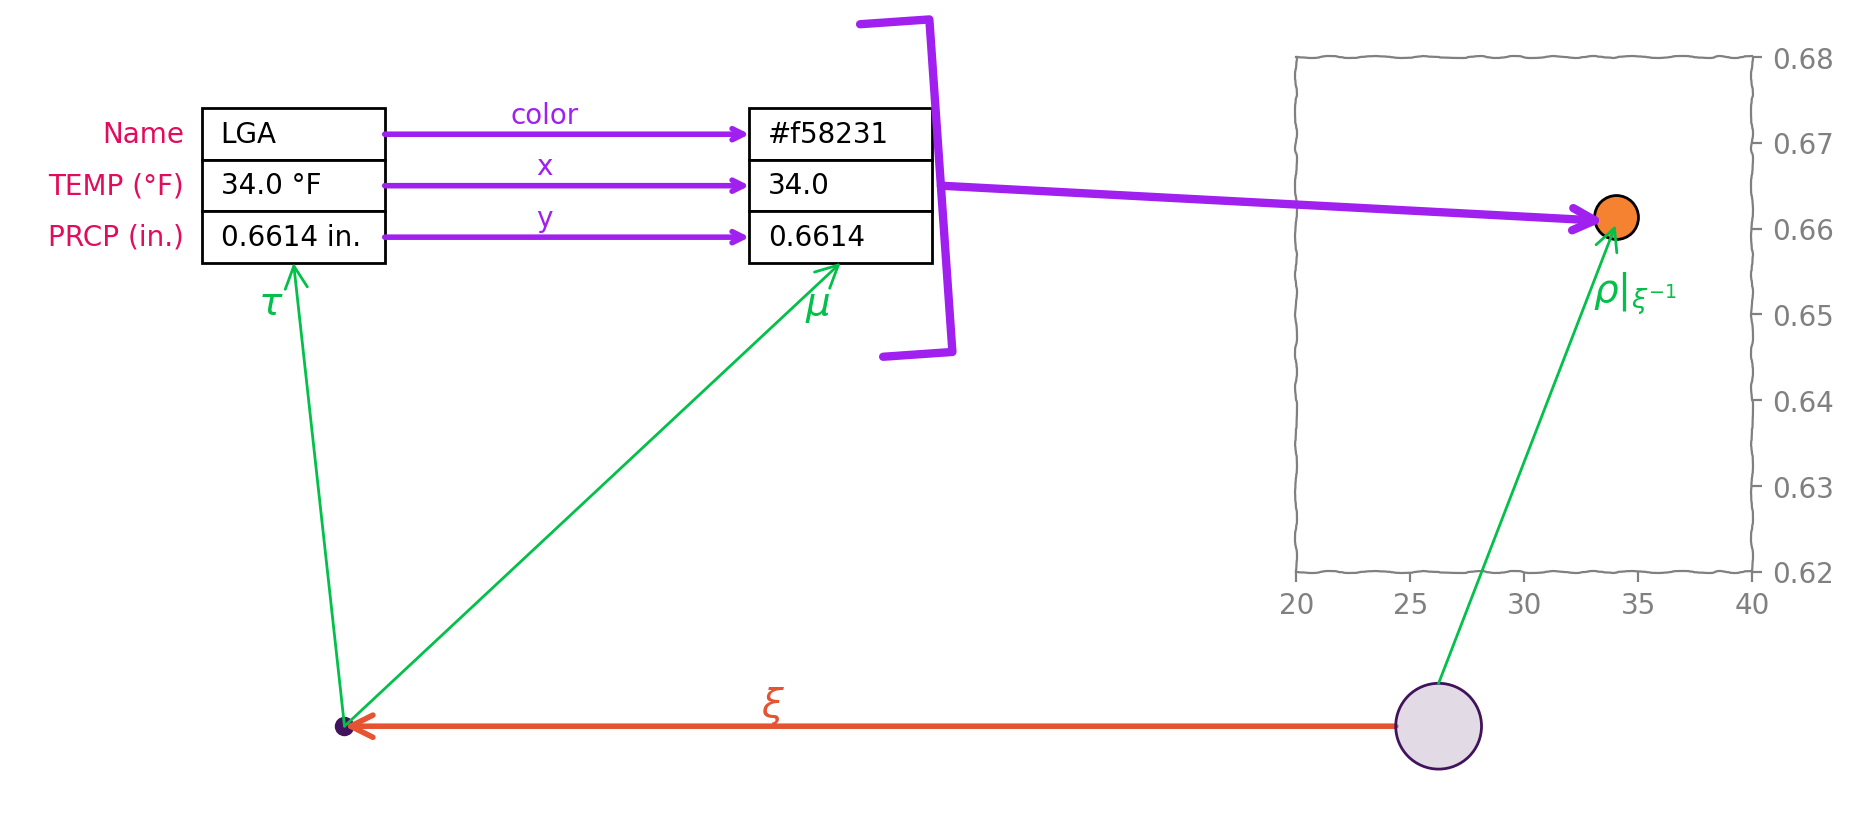
\includegraphics[width=1\columnwidth]{full_scatter.png}
  \caption{This simple $\vmarkc$ assembles a circular visual element that is the color specified in $\vsection(\dbasepoint)$ and is at the intersection specified in $\vsection(\dbasepoint)$ \label{fig:construction:q} \note{much better labeling, include semantic labeling, make everything bigger}}
\end{figure}
As shown in \autoref{fig:construction:q}, a set of  $\vchannel$ functions individually convert the values in the data record to visual components. Then the $\vmark$ function combines these visual encodings to produce a graphic section \gsection. When this section is evaluated on the graphic space associated with the data $\gsection(\vindexpre(\dbasepoint))$, it produces a blue circular marker at the intersection of the x and y positions listed in \vsection. The composition rule in \autoref{eq:construction:q:fabrication} means that developers can implement $\vmark$ as drawing circles or can implement a $\vmark$ that draws arbitrary shapes, and then provide different $\vchannel$ adapters, such as one that specifies that the shape is a circle. 

\subsubsection{Compositor Verification}
\label{sec:construction:q:verification}
An advantage of factoring out encoding and verification, as discussed in \autoref{sec:construction:nu:verification}, is that the responsibility of the compositor can be scoped to translating measurable components into visual elements. 
\begin{equation}
  \label{eq:construction:q:validate}
  \begin{tikzcd}[row sep=huge]
    \cgamma{\dbasec}{\vtotalc^{a}\times \vtotalc^{b}}  
    \arrow[rr, "\vmarkc_{ab}", color=artist] 
    \arrow[d, "\pi_a"', color=total] &  &  \imartistsub{ab}{\gbasec}{\gtotalc} 
    \arrow[d, "\measurec\restriction_a \circ \extractmc_{ab}", color=monoid]  \\
   \cgamma{\dbasec}{\vtotalc^{a}} 
   \arrow[rr, "\simeq", dotted] &  & 
   {\textcolor{set}{Hom}(\dbasec, \measurec^{a})}  \\
    \cgamma{\dbasec}{\vtotalc^{a}\times \vtotalc^{c}}  
    \arrow[rr, "\vmarkc_{ac}", color=artist] 
    \arrow[u, "\pi_a", color=total]  &  &  \imartistsub{ac}{\gbasec}{\gtotalc} 
    \arrow[u, "\measurec\restriction_a \circ \extractmc_{ac}"', color=monoid]
   \end{tikzcd}
\end{equation}
As illustrated in \autoref{eq:construction:q:validate}, a compositor is valid if there is an isomorphism between the actual outputted measured visual component and the expected measurable component that is the input. One way of verifying that a compositor is consistent is by verifying that it passes through one encoding even while changing others. For example, when $\vmark_{ab}=\vmark_{ac}$ then the output should differ in the same measurable components as $\vsectionc_{ab}$ and $\vsection_{ac}$. 

A compositor function \vmark\ is equivariant if the renderer output changes in a way equivariant to the data transformation defined in \autoref{sec:artist:equivariant:data}. This means that a change in base space $\dfunch_{\dtotalc}$ should have an equivalent change in visual element base space. This means that there should be no change in visual measurement
\begin{equation}
  \label{eq:construction:q:verification:base}
  \vsectionc(\dfunchc_{\dbasec}(\dbasepointc^{\prime})) = \extractmc(\vmarkc(\vsectionc)(\dfunch_{\dbasec}(\vindexprec^{\dbasepointc}))) = \measurec_{\dbasepointc}
\end{equation}
As discussed in \autoref{fig:artist:equivariance}, the change in base space may induce a change in locations of measurements relative to each other in the output; this can be verified via checking that all the measurements have not changed relative to the original positions $\measurec_{\dbasepoint} = \measurec_{\dbasepointc^{\prime}}$ and through separate measurable variables that encode holistic data properties, such as orientation or origin. 

The compositor function is also expected to be equivariant with respect to changes in data and measurable components
\begin{equation}
  \label{eq:construnction:q:verify:base}
  \dfunctc_{\vtotalc}(\vsectionc(\dbasepointc)) = \dfunctc_{\measurec}(\vmarkc(\vsectionc(\dbasepointc)))  
\end{equation}
which means that any change to a measurable component input must have a measurably equivalent change in the output. As illustrated in \autoref{fig:artist:equivariance}, the compositor $\vmarkc$ is expected to assemble the measurable components such that base space changes, for example transposition, are reflected in the output; faithfully pass through equivariant measurable components, such as scaled colors; and ensure that both types of transformations, here scaling and transposition, are present in the final glyph.  

\subsection{Implementing the Artist}

 When a sheaf is equipped with transport functors, then the functions between sheaves over one space are isomorphic to functions between sheaves over the other space\cite{harder2008lectures} such that the following diagram commutes

 \note{should either be oriented same as 55 and/or pushed back up to 3.3 as an intro to artist or squished a little. }
 \begin{equation}
  \label{eq:atct:sheaves:homset}
  \begin{tikzcd}
    \cgamma{\opensetc}{\dtotalc\restriction_{\opensetc}} 
    \arrow[dd, "\textcolor{set}{Hom}_{\sheafc_{\dbasec}}"', color=homset] 
    \arrow[rrdd, "\textcolor{set}{Hom}_{\sheafc_{\dbasec},\sheafc_{\gbasec}}", color=homset] 
    \arrow[rr, "\vindexpullc", color=functor] &  &
    \cgamma{\opensetgc}{\vindexpullc\dtotalc\restriction_{\opensetgc}} 
    \arrow[dd, "\textcolor{set}{Hom}_{\sheafc_{\gbasec}}", color=homset] \\
     & & \\
    \cgamma{\opensetc}{\vindexpushc\gtotalc\restriction_{\opensetc}} &  & 
    \cgamma{\opensetgc}{\gtotalc\restriction_{\opensetgc}} 
    \arrow[ll, "\vindexpushc"', color=functor]                  
    \end{tikzcd}
\end{equation}

Since the artist is a family of functions in the homset between sheaves, the isomorphism allows for the specification of the transformation from data as combination of functions over different spaces such that the following diagram commutes:
\begin{equation}
  \label{eq:construction:artist:path}
\begin{tikzcd}[row sep=2.5em, column sep=1.5em]
  \cgamma{\dbasec}{\dtotalc} 
  \arrow[rr, "\vchannelc^{\dbasec}", color=artist] 
  \arrow[rrrr, "\vartistc^{\dbasec}", bend left, color=artist] 
  \arrow[dd, "\vindexpullc"', color=functor] 
  \arrow[rrrrdd, "\vartistc", color=artist, pos=.2] &  & 
  \cgamma{\dbasec}{\vtotalc} 
  \arrow[rrdd, "\vmarkc", color=artist] 
  \arrow[rr, "\vmarkc^{\dbasec}", color=artist] 
  \arrow[dd, "\vindexpullc", color=functor, pos=.2] &  & \imartist{\dbasec}{\vindexpushc\gtotalc}  \\
   & & & & \\
  \cgamma{\gbasec}{\vindexpullc\dtotalc} 
  \arrow[rr, "\vchannelc^{\gbasec}", color=artist] 
  \arrow[rrrr, "\vartistc^{\gbasec}", bend right, color=artist] & & 
  \cgamma{\gbasec}{\vindexpullc\vtotalc} 
  \arrow[rr, "\vmarkc^{\gbasec}", color=artist] &  & 
  \imartist{\gbasec}{\gtotalc} 
  \arrow[uu, "\vindexpushc"', color=functor]
\end{tikzcd}  
\end{equation}
This means that an artist over data space $\vartist_{\dbase}: \dsection \mapsto \vindexpush \gsection$, an artist over graphic space $vartist_{\gbase}: \vindexpull \dsection \mapsto \gsection$, and an artist $\vartist: \dsection \mapsto \gsection$ are equivalent such that:
\begin{equation*}
  \begin{split}
  & \dsection(\dbasepoint) = \vindexpull\dsection(\gbasepoint)  \\
   & \implies
  \vartist_{\dbase}(\dsection(\dbasepoint)) = \vartist_{\gbase}(\vindexpull\dsection(\gbasepoint)) = \vartist(\dsection(\dbasepoint))\\
  & \implies \vindexpush\gsection(\gbasepoint) = \gsection(\gbasepoint) 
  \end{split}
\end{equation*}
when $\vindex(\gbasepoint) = \dbasepoint$. This equivalence allows a  developer to connect transformations over data space, denoted with a subset $\dbase$, with transformations over graphic space $\gbase$, using $\vindexpushc$ and $\vindexpullc$ adaptors.This allows developers to for example connect transformers that transform data on a line to a color in data space, but build a line compositing function that dynamically resamples what is on screen in graphic space.


\section{Discussion: Feasibility as Design Spec}
\label{sec:discussion}

The framework specified in \autoref{sec:artist} and \autoref{sec:construction} describes how to build structure preserving visualization components, but it is left to the library developer to follow these guidelines when building and reusing components. In this section, we introduce a toy example of building an artist out of the components introduced in \autoref{sec:construction} to illustrate how components that adhere to these specifications are maintainable, extendible, scalable, and support concurrency. 

\begin{figure}[H]
  \centering
  \subfloat[]{
    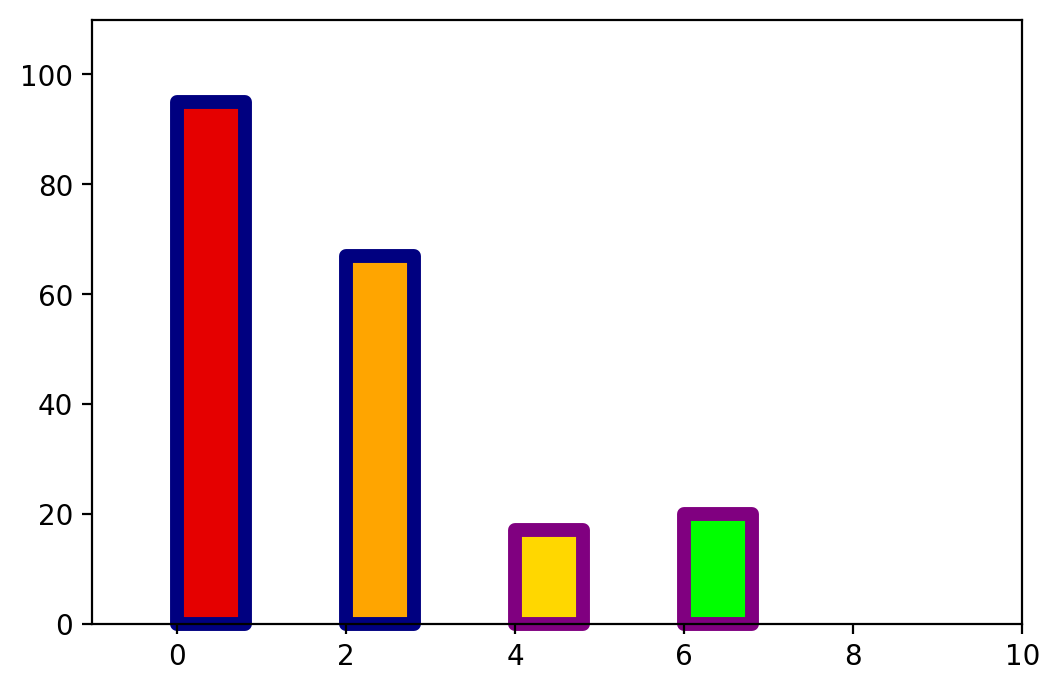
\includegraphics[width=.45\columnwidth]{bar.png}
  \label{fig:discussion:vbar}}
  \subfloat[]{
    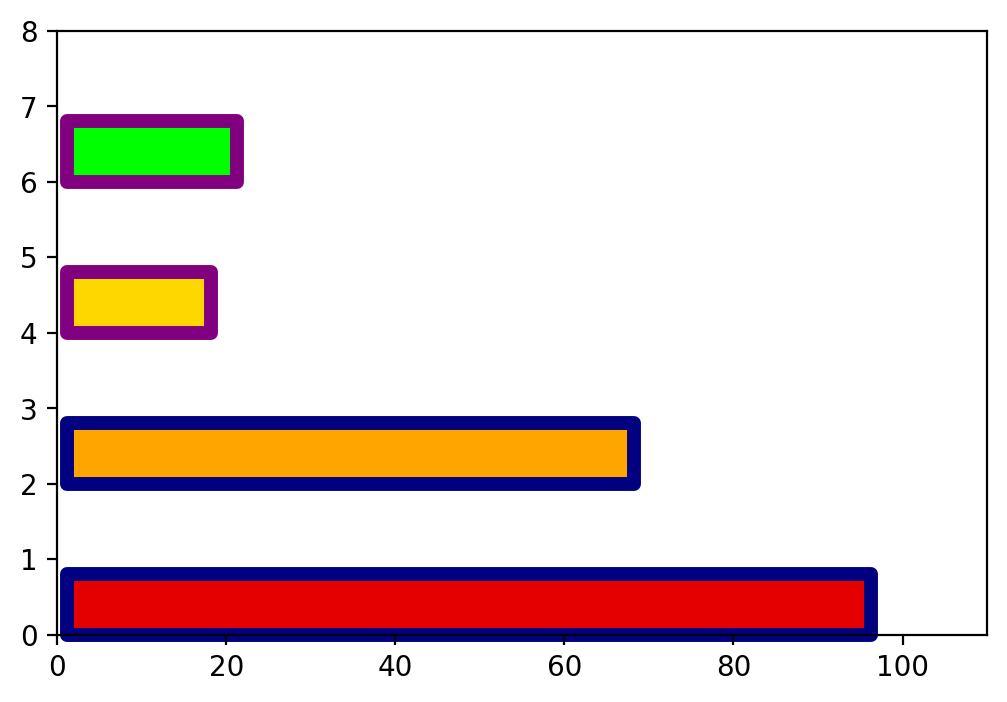
\includegraphics[width=.45\columnwidth]{barh.png}
  \label{fig:discussion:hbar}
  }
  \label{fig:discussion:bar}
\end{figure}

Specially, we introduce artists for building the graphical elements shown in \autoref{fig:discussion:bar} because it is a visualization type that allows us to demonstrate composability and multivariate data encoding. We build our visualization components by extending the Python visualization library Matplotlib's artist\footnote{Matplotlib artists are our artist's namesake}\cite{hunterMatplotlib2DGraphics2007,hunterArchitectureOpenSource} to show that components using this model can be incorporated into existing visualization libraries iteratively. While the architecture specified in \autoref{sec:construction} can be implemented fully functionally, we make use of objects to keep track of parameters passed into artists. In this toy example, the small composable components allow for more easily verifying that each component does its transformation correctly before assembling them into larger systems.  

\subsection{Bundle Inspired Data Containers}
\begin{table}[H]
  \centering
\begin{tabular}{|lcl|}
  \hline \\
   fruit &  calories &  juice \\
  \hline\\
    apple &        95 &   True \\ 
   orange &        67 &   True \\ 
  lemon &        17 &  False \\ 
      lime &        20 &  False \\
  \hline
\end{tabular}
\label{tab:discussion:data}
\end{table}
We construct a toy dataset with a discrete $\dbase$ of 4 points and a fiber space of $\dfiber=\{apple,\, orange,\, lemon\}\times \mathbb{Z}^{+} \times \{\texttt{True}, \texttt{False}\}$. We thinly wrap \autoref{tab:discussion:data} in an object so that the common data interface function is that $\tau = \texttt{DataContainerObject.query}$. 
\begin{minted}{python}
  class FruitFrameWrapper:
    def query(self, data_bounds, sampling_rate):
      # local sections are a list of
      # {field: local_batch_of_values}
      return local_sections
\end{minted}

This interface provides a uniform way of accessing subsets of the data, which are local sections. The motivation for a common data interface is that it would allow the artist to talk to different common python data containers, such as numpy\cite{harris2020array}, pandas\cite{jeff_reback_2020_3715232}, xarray \cite{hoyer2017xarray}, and networkx\cite{HagbergExploringNetwork2008}. Currently, data stored in these containers must be unpacked and converted into arrays and matrices in ways that either destroy or recreate the structure encoded in the container. For example a pandas data frame must be unpacked into its columns before it is sent into most artists and continuity is implicit in the columns being the same length rather than a tracked base space $\dbase$. Because it is more efficient to work with the data in column order, we often project the fiber down into individual components. As shown in \autoref{eq:atct:fiber_product}, we can verify that this projection is correct by checking that the values at the index are the same regardless of the level of decomposition. 

\subsection{Component Encoders}
To encode the values in the dataset, we enforce equivariance by writing $\vchannel$ encoders that match the structure of the fields in the dataset. For example, the fruit column is a nominal measurement scale. Therefore we implement a position encoder that respects permutation $\dfunch$ transformations. The most simple form of this $\vchannel$ is a python dictionary that returns an integer position, because Matplotlib's internal parameter space expects a numerical position type. 
\begin{minted}{python}
  def position_encoder(val):
    return {'apple': 0, 'orange': 2, 'lemon': 4, 'lime': 6}[val]
\end{minted}
As mentioned in \autoref{eq:construction:nu:fabrication}, the encoders can be composed up. For example, the compositor $\vchannel$ may need the position to be converted to screen coordinates. Here the screen coordinate $\vchannel$ is a method of a Matplotlib axes object; a Matplotlib axes is akin to a container artist that holds all information about the sub artists plotted within it. 
\begin{minted}{python}
def composite_x_transform(ax, nu):
    return lambda x: ax.transData.transform(
            (position_encoder(x), 0))[0]
\end{minted}
This encoder returns a function that is \texttt{transData.transform} $\vchannel_{transData}$ composed with the position encoder $\vchannel_{position}$ and takes as input a record to be encoded. As with the position encoder, the transData encoder respects permutation transforms because it returns reals; therefore the composite encoder respects permutation transforms. In this model, developers implement $\vchannel$ encoders that are explicit about which $\dfunc_{\vtotal}$ they support. Writing semantically correct encoders is also the responsibility of the developer and is not addressed in the model. For example \mintinline{python}{fruit_encoder = lamda x: {'apple': green, 'orange':'yellow', 'lemon':'red', 'lime':'orange'}} is a valid color encoding with respect to permutation, but none of those colors are intuitive to the data. It is therefore left to the user, or domain specific library developer, to choose $\vchannel$ encoders that are appropriate for their data.

\subsection{Graphic Compositors}
After converting each record into an intermediate visual component $\vsection$, the set of visual records is passed into $\vmarkc$. Here the $\vmarkc$ includes one last encoder, as illustrated in \autoref{eq:construction:q:fabrication}, that assembles the independent visual components into a rectangle. This $\vchannel$ is inside the $\vmarkc$ to hide that library preferred format from the user. It is called \texttt{qhat} to indicate that this is the $\vartist^{\dbase}$ path in \autoref{eq:construction:artist:path}.  This means that the parameters are constructed in data space $\dbase$ and this function returns a pushed forward $\vindexpush\gsection$. 

\begin{minted}{python}
   def qhat(position, width, length, floor, facecolor, edgecolor, linewidth, linestyle): 
        box = box_nu(position, width, length, floor)
        def fake_draw(render, transform=mtransforms.IdentityTransform()):
            for (bx, fc, ec, lw, ls) in zip(box, facecolor, edgecolor, linewidth, linestyle):
                gc = render.new_gc()
                gc.set_foreground((ec.r, ec.g, ec.b, ec.a))
                gc.set_dashes(*ls)
                gc.set_linewidth(lw)
                render.draw_path(gc=gc, path=bx, transform=transform, rgbFace=(fc.r, fc.g, fc.b, fc.a))
        return fake_draw
\end{minted}
The function \texttt{fake\_draw} is the analog of $\vindexpush\gsection$. This function builds the rendering spec through the renderer API, and this curried function is returned. The transform here is required for the code to run, but is set to identity meaning that this function directly uses the output of the position encoders. The curried $\texttt{fake\_draw} \approx \vindexpush \gsection$ is evaluated using a renderer object. In our model, as shown in \autoref{eq:artist:inout:diagram}, the renderer is supposed to take $\gsection$ as input such that $renderer(\gsection) = visualization$, but here that would require an out of scope patching of the Matplotlib render objects. 

One of the advantages of this model is that it allows for succinctly expressing the difference between two very similar visualizations, such as \autoref{fig:discussion:vbar} and \autoref{fig:discussion:hbar}. In this model, the horizontal bar is implemented as a composition of a $\vchannel$ that renames fields in $\vsection_{barh}$ and the $\vmark$ implementation for the horizontal bar.
\begin{minted}{python}
def qhat(length, width, position, floor, facecolor, edgecolor, linewidth, linestyle):
  return Bar.qhat(**BarH.bar_nu(length, width, position, floor, facecolor, edgecolor, linewidth, linestyle))
\end{minted}
This composition is equivalent to $\vmark_{barh} = \vmark_{bar} \circ \vchannel_{vtoh}$, which is an example of \autoref{eq:construction:q:fabrication}. These functions can be further added together, as described in \autoref{sec:artist:operators} to build more complex visualizations. 

\subsection{Integrating Components into an Existing Library}
The $\vchannel$ and $\vmark$ are wrapped in a container object that stores the $\vartist = \vmark \circ \vchannel$ composition and a method for computing the $\vsectionc$.
\begin{minted}{python}
  class Bar: 
    def compose_with_nu(self, pfield, ffield, 
          nu, nu_inv:):
        # returns a new copy of the Bar artist 
        # with the additional nu that converts 
        # from a data (F) field value to a 
        # visual (P) field value
        return new

    def nu(self, tau_local): #draw
       # uses the stored nus to convert data
       # stored nus have F->P field info
      return mus
    
    @staticmethod
    def qhat(position, width, length, floor, facecolor, edgecolor, linewidth, linestyle):
       
        return fake_draw
\end{minted}

As shown in the \texttt{draw} method, generating a graphic section $\gsection$ is implemented as the composition of $\texttt{qhat} \approx \vmark$ and $\texttt{nu} \approx \vchannel$ applied to a local section of the sheaf $\texttt{self.section.query} \approx \dsection^{i}$ such  $\texttt{draw} \approx \vmarkc\circ\vchannelc\circ\dsectionc  = \vartistc\circ \dsectionc$. The $\vchannel$ and $\vmark$ functions shown here are written such that they can generate a visual element given a local section $\dsection\restriction_{\dbase^{i}}$ which can be as little or large as needed. This flexibility is a prerequisite for building scalable and streaming visualizations that may not have access to all the data.  

This artist is then passed along to a shim artist that makes it compatible with existing Matplotlib objects (\autoref{sec:appendix:artist_shim}). This shim object is hooked into the Matplotlib draw tree to produce the vertical bar chart in \autoref{fig:discussion:vbar}. Using the Matplotlib artist framework means this new artist can be composed with existing artists, such as the ones that draw the axes and ticks. The example in this section is intentionally trivial to illustrate that the math to code translation is fairly straightforward and results in fairly self contained composable functions. A library applying these ideas, created by Thomas Caswell, can be found at \url{https://github.com/matplotlib/data-prototype}. Further research could investigate building new systems using this model, specifically libraries for visualizing domain specific structured data and domain specific artists. More research could also explore applying this model to visualizing high dimensional data, particularly building artists that take as input distributed data and artists that are concurrent. Developing complex systems could also be an avenue to codify how interactive techniques are expressed in this framework.

\section{Conclusion}
The toy example presented in \autoref{sec:discussion} demonstrates that it is relatively straightforward to build working visualization library components using the construction described in \autoref{sec:construction}. Since these components are defined with single record inputs, the can be implemented such that they are concurrent. The cost of building a new function using these components is sometimes as small as renaming fields, meaning the new feature is relatively easy to maintain. These new components are also a lower maintenance burden because, by definition, they are designed in conjunction with tests that verify that they are equivariant.  
These new components are also compatible with the existing library architecture, allowing for a slow iterative transition to components built using this framework. 
The framework introduced in this paper is a marriage of the ways the graphic and data visualization communities approach visualization. The graphic community prioritizes \note{?} how input is translated to output, which is encapsulated in the artist $\vartist$. The data visualization community prioritizes the manner in which that input is encoded, which is encapsulated in the separation of stages $\vmark \circ \vchannel$. Formalizing that both views are equivalent $\vartist=\vmark \circ \vchannel$ gives library developers the flexibility to build visualization components in the manner that makes more sense for the domain without having to sacrifice the equivariance of the translation. 

\appendices

\section{Summary}
\label{sec:appndix:summary}
The topological spaces and functions introduced throughout this paper are summarized here for reference. 

\begin{table}[H]
  \centering
  {\renewcommand{\arraystretch}{1.5}
  \begin{tabular}{|r | c c c|}
    \hline
    &\textcolor{base}{point}/\textcolor{base}{openset}/\textcolor{base}{base space} & \textcolor{fiber}{fiber space} & \textcolor{total}{total space}\\
     &  location/subset/indices & record/fields &  dataset type\\
    \hline
   Data & $\dbasepointc \in \opensetc \subseteq \dbasec$ & $\delementc \in \dfiberc$ & \dtotalc\\
   Visual & $\dbasepointc \in \opensetc \subseteq \dbasec$  & $\velementc \in \vfiberc$ & \vtotalc\\
   Graphic & $\gbasepointc \in \opensetgc \subseteq \gbasec$ & $\gelementc \in \gfiberc$ & \gtotalc\\
   \hline
  \end{tabular}
  \caption{Topological spaces introduced in \autoref{sec:atct:fiber-bundles}}
  \label{tab:appendix:summary:objects}
  }
\end{table}

\begin{table}[H]
  \centering
  {\renewcommand{\arraystretch}{1.5}
  \begin{tabular}{|r | l l | }
    \hline
     & \textcolor{section}{section} & \textcolor{sheaf}{sheaf} \\
     & record at location & set of possible records for subset \\
     \hline
  Data & $ \cgamma{\dbasec}{\dtotalc} \ni \dsectionc: \dbase \textcolor{section}{\rightarrow} \dfiberc$ & $\sheafc_{\dbasec, \dtotalc}: \opensetc \rightarrow \cgamma{\opensetc}{\dtotalc\restriction_{\opensetc}}$\\
  Visual &  $\cgamma{\dbasec}{\vtotalc} \ni \vsectionc: \dbase \textcolor{section}{\rightarrow} \vfiberc$ & $\sheafc_{\dbasec, \vtotalc}: \opensetc \rightarrow \cgamma{\opensetc}{\vtotalc\restriction_{\opensetc}}$\\
  Graphic &    $\cgamma{\gbasec}{\gtotalc} \ni \gsectionc: \gbase \textcolor{section}{\rightarrow} \gfiberc$ &  $\sheafc_{\gbasec, \gtotalc}: \opensetgc \rightarrow \cgamma{\opensetc}{\gtotalc\restriction_{\opensetgc}}$ \\ 
  \hline
  \end{tabular}
  \caption{Functions that associate topological subspaces with records, discussed in \autoref{sec:atct:fb:sections} and \autoref{sec:atct:sheaves}}
  \label{tab:appendix:summary:datafunctions}
  }
\end{table}

\begin{table}[H]
  \centering
  {\renewcommand{\arraystretch}{1.5}
  \begin{tabular}{|r | l  l |}
\hline
& function & constraint\\
\hline
 \gbasepointc\ to \dbasepointc& $ \vindexc: \opensetgc \rightarrow \opensetc$ & for $\gbasepointc \in \opensetgc$ exists $\dbasepointc \in \opensetc$ \\
 & & s.t. $\vindexc(\gbasepointc) = \dbasepointc$\\
 graphic for \dbasepointc & $ \vindexpushc \gsectionc: \opensetc \rightarrow \vindexpushc\gtotalc\restriction_{\opensetc}$ & $\vindexpushc\gsectionc(\dbasepointc)(\gbasepointc) = \gsectionc(\gbasepointc)$ \\
 record for \gbasepointc & $\vindexpullc\dsectionc: \opensetgc \rightarrow  \vindexpullc\dtotalc\restriction_{\opensetgc}$ & $\vindexpullc\dsectionc(\gbasepointc)=\dsectionc(\vindexc(\gbasepointc)) = \dsectionc(\dbasepointc)$  \\
\hline
  \end{tabular}
  \caption{Functors between graphic and data indexing spaces  \autoref{sec:atct:xi}}
  \label{tab:appendix:summary:transport}
  }
\end{table}

\begin{table}[H]
\centering
{\renewcommand{\arraystretch}{1.5}
\begin{tabular}{|r|l|l|}
  \hline
  changes & function & constraints, for all $\dbasepointc \in \opensetc$ \\
  \hline
  index & $\dfunchc: \opensetc \rightarrow \opensetc^{\prime}$ &   $\dsectionc(\dbasepointc) = \dsectionc(\dfunchc(\dbasepointc^{\prime})) = \dfuncpullc \dsectionc(\dbasepointc^{\prime})$ \\
  & & \\
  record  & $\dfunctc: \cgamma{\opensetc^{\prime}}{\dfuncpullc\dtotalc\restriction_{\opensetc}}$ &  $\lim\limits_{x\rightarrow \dbasepointc}\dfunctc(\dsectionc(x)) = \dfunctc(\dsectionc(\dbasepointc))$
  \\
  & $\textcolor{white}{\dfunct: } \rightarrow \cgamma{\opensetc^{\prime}}{\dfuncpullc\dtotalc\restriction_{\opensetc}}$ &    
  \\
  & $\dfunctc: \dfiberc \rightarrow \dfiberc$ &  $\dfunctc(\dsectionc(\dbasepointc)) \in \dfiberc$  \\ 
  & & $\dfunctc(id_{\dfiberc}(\dsectionc(\dbasepointc))) = id_{\dfiberc}(\dfunctc(\dsectionc(\dbasepointc)))$\\
  & & $\dfunctc(\dfunctc(\dsectionc(\dbasepointc))) = (\dfunctc\circ\dfunctc)(\dsectionc(\dbasepointc))$\\
  \hline
\end{tabular}
\caption{Functions $\dfunc=(\dfunchc, \dfunctc)$ for modifying data records. Equivalent constructions can be applied to elements in visual and graphic sheaves, and these functions are distinguished through subscripts $\dfunc_{\dtotal}$, $\dfunc_{\vtotal}$ and $\dfunc_{\gtotal}$}
\label{tab:appendix:summary:datamod}
}
\end{table}

\begin{table}[H]
  \renewcommand{\arraystretch}{1.5}
  \begin{tabular}{|lll|}\hline
      scale & operators & sample constraint \\ \hline
      nominal & $=,\neq$ &  $\dsectionc(\dbasepointc_1) \neq \dsectionc(\dbasepointc_2)\implies \dfunctc (\dsectionc(\dbasepointc_1)) \neq\dfunctc(\dsectionc(\dbasepointc_2))$\\ 
      ordinal & $<, \leq, \geq, >$ &  $\dsectionc(\dbasepointc_1) \leq \dsectionc(\dbasepointc_2) \implies \dfunctc (\dsectionc(\dbasepointc_1)) \leq \dfunctc(\dsectionc(\dbasepointc_2)$) \\
      interval & $+, -$ &  $\dfunctc(\dsectionc(\dbasepointc) + C) = \dfunctc(\dsectionc(\dbasepointc)) + C$ \\
      ratio & $*,/$ &  $\dfunctc(\dsectionc(\dbasepointc) * C) = \dfunctc(\dsectionc(\dbasepointc))*C $\\ \hline
  \end{tabular}
  \caption{The record transformer $\dfunctc$ must satisfy the constraints listed in \autoref{tab:appendix:summary:datamod} and $\dfunctc$ must also respect the mathematical structure of $\dfiber$. This table lists examples of $\dfunct$ preserving one of the binary operators that are part of the definition of each of the Steven's measurement scale types\cite{stevensTheoryScalesMeasurement1946}}. A full implementation would ensure that all operators that are defined as part of of $\dfiber$ are preserved.  
  \label{tab:appendix:summary:stevens}
\end{table}

\begin{table}[H]
  \centering
  {\renewcommand{\arraystretch}{1.2}
\begin{tabular}{|r|l|l|}
  \hline
      & function & constraints \\
  \hline
  \textcolor{artist}{artist} & $\vartistc: \cgamma{\dbasec}{\dtotalc} \rightarrow \imartist{\gbasec}{\gtotalc}$ &  \\
  Data to Graphic  &  $\imartist{\gbasec}{\gtotalc} \subset \cgamma{\gbasec}{\gtotalc}$ & $\vindexc(\gbasec) = \dbasec$\\
  & & \\
  \hline 
  Encode
    & & \\
           & & \\
  \hline
  Decompose & & \\
              && \\
  \hline
\end{tabular}
\caption{artist, verification functions, and construction $\vartist = \vmarkc \circ \nu$ introduced in \autoref{sec:artist}, and \autoref{sec:construction}}
\label{tab:appedendix:summary:artist}
}
\end{table}


\note{color}
\begin{table}[H]
  \centering
  {\renewcommand{\arraystretch}{1.2}
\begin{tabular}{|r|l|l|}
  \hline
      & function & constraint \\
  \hline
  \textcolor{artist}{artist} & $\vartist: \Gamma(\dbase, \dtotal) \rightarrow \Gamma(\gbase, \gtotal)$ &  \\
  \hline 
  \textcolor{functor}{lookup} & $\vindex: \gbase\rightarrow \dbase$  &  \\ 
  \hline
  \textcolor{artist}{encoders} & $\vchannel: \Gamma(\dbase, \dtotal) \rightarrow \Gamma(\dbase, \vtotal) $  & \\
  \hline
  \textcolor{artist}{compositor} & $\vmark: \Gamma(\dbase,\vtotal) \rightarrow \Gamma(\gbase, \vtotal)$ &  \\
  \hline
\end{tabular}
\caption{artist, verification functions, and construction $\vartist = \vmarkc \circ \nu$ introduced in \autoref{sec:artist}, and \autoref{sec:construction}}
\label{tab:appendix:summary:artist}
}
\end{table}

\pagebreak
\section{Internal Library Specification}

\label{tab:appendix:library_spec}
\begin{table}[H]
  \centering
  \renewcommand{\arraystretch}{2}
  \begin{tabulary}{\columnwidth}{|l|L|l|}\hline
   \(\bm{\vchannel_{i}}\)    & \(\bm{\vsection_{i}}\)  & \(\bm{codomain(\vchannel_{i}) \subset \vfiber_{i}}\)  \\ \hline                                              
  position                    & x, y, z, theta, r      & \(\mathbb{R}\)   \\ \hline
  size                        & linewidth, markersize  & \(\mathbb{R}^{+}\)  \\ \hline
  shape                       & markerstyle            & \(\{f_{0}, \ldots, f_{n}\}\)\\ \hline
  color                       & color, facecolor, markerfacecolor, edgecolor  & \(\mathbb{R}^{4}\) \\ \hline
  \multirow{2}{*}{texture}    & hatch      & \(\mathbb{N}^{10}\)\\\cline{2-3}
                              & linestyle    & \((\mathbb{R}, \mathbb{R^+}^{n, n\%2=0})\) \\ \hline              
  \end{tabulary}
  \caption{Some of the $\vfiber$ components of the $\vtotal$ bundles in Matplotlib components}
  \label{tab:math:artist:mpl:fiber}
\end{table}

\pagebreak
\section{Matplotlib Compatibility}
\label{sec:appendix:artist_shim}

As mentioned in \autoref{sec:discussion}, one advantage of using this type of  
functional categorical approach to software design is that we can develop new 
components that can be incorporated into the existing code base. For matplotlib, 
we can use these functional artists by wrapping them in a very thin compatibility
layer shim so that they behave like existing artists. 

\begin{minted}{python}
  class GenericArtist(martist.Artist):
      def __init__(self, artist:TopologicalArtist):
          super().__init__()
          self.artist = artist
          
      def compose_with_tau(self, section):
          self.section = section
  
      def draw(self, renderer, bounds, rate):
          for tau_local in self.section.query(bounds, rate): 
              mu = self.artist.nu(tau_local)
              rho = self.artist.qhat(**mu)
              output = rho(renderer)
  \end{minted}
% use section* for acknowledgment

\section*{Acknowledgment}
\note{Acknowledge all the actual people}
The authors would like to thank...

Hannah is also very grateful to the nlab and wikipedia contributors who wrote 
articles explaining a lot of the more abstract math on which this paper is built. 

% Can use something like this to put references on a page
% by themselves when using endfloat and the captionsoff option.
\ifCLASSOPTIONcaptionsoff
  \newpage
\fi

% trigger a \newpage just before the given reference
% number - used to balance the columns on the last page
% adjust value as needed - may need to be readjusted if
% the document is modified later
%\IEEEtriggeratref{8}
% The "triggered" command can be changed if desired:
%\IEEEtriggercmd{\enlargethispage{-5in}}

% references section

% can use a bibliography generated by BibTeX as a .bbl file
% BibTeX documentation can be easily obtained at:
% http://mirror.ctan.org/biblio/bibtex/contrib/doc/https://www.overleaf.com/download/project/64063771726807fc06c1ee16/build/187faee483d-291434de4cddeda6/output/output.pdf?compileGroup=priority&clsiserverid=clsi-pre-emp-c2d-d-f-nkpv&enable_pdf_caching=true&popupDownload=truejjj
% The IEEEtran BibTeX style support page is at:
% http://www.michaelshell.org/tex/ieeetran/bibtex/

\bibliographystyle{IEEEtran}
% argument is your BibTeX string definitions and bibliography database(s)
\bibliography{references}

% biography section 
% If you have an EPS/PDF photo (graphicx package needed) extra braces are
% needed around the contents of the optional argument to biography to prevent
% the LaTeX parser from getting confused when it sees the complicated
% \includegraphics command within an optional argument. (You could create
% your own custom macro containing the \includegraphics command to make things
% simpler here.)
%\begin{IEEEbiography}[{\includegraphics[width=1in,height=1.25in,clip,keepaspectratio]{mshell}}]{Michael Shell}
% or if you just want to reserve a space for a photo:

%\begin{IEEEbiography}{Michael Shell}
%\end{IEEEbiography}

% if you will not have a photo at all:
\begin{IEEEbiographynophoto}{Hannah Aizenman}
Biography text here.
\end{IEEEbiographynophoto}

\begin{IEEEbiographynophoto}{Thomas Caswell}
  Biography text here.
\end{IEEEbiographynophoto}
% insert where needed to balance the two columns on the last page with
% biographies
%\newpage

\begin{IEEEbiographynophoto}{Michael Grossberg}
Biography text here.
\end{IEEEbiographynophoto}

% You can push biographies down or up by placing
% a \vfill before or after them. The appropriate
% use of \vfill depends on what kind of text is
% on the last page and whether or not the columns
% are being equalized.

%\vfill

% Can be used to pull up biographies so that the bottom of the last one
% is flush with the other column.
%\enlargethispage{-5in}

% that's all folks
\end{document}


